\documentclass[12pt]{article}
\usepackage{float}
\usepackage{listings}
\usepackage{amsthm}
\usepackage{amsmath}
\usepackage{lineno}
\usepackage{cite}
\usepackage{amssymb,graphics,color,cite,amsmath}
\usepackage{subfig}
\usepackage{graphicx}
\usepackage{epsfig}
\usepackage{psfrag}
\usepackage[margin=0.75in]{geometry}
\usepackage{float}
\usepackage{afterpage}
\usepackage{hyperref}
\usepackage{verbatim}
\usepackage{enumitem}
\setlist[itemize]{topsep=0pt,after=\vspace{1.\baselineskip}}

\usepackage[noblocks]{authblk}
%\usepackage{natbib}
\usepackage{stackengine}

\usepackage{xspace}
\newcommand{\themename}{\textbf{\textsc{metropolis}}\xspace}

\renewcommand{\(}{\left (}
\renewcommand{\)}{\right )}
\renewcommand{\vec}[1]{\boldsymbol{#1}}

\begin{document}

\title{Synchronization of Two Cellular Circadian Rhythms}
\date{}
\author[1]{Zeshun Zong}
\author[2]{Yuliang Shi}
\affil[1,2]{\footnotesize Courant Institute of Mathematical Sciences, New York University, New York}


\maketitle
\begin{abstract}
ABSTRACT
\end{abstract}

\section{Introduction}

\hspace{5mm} Almost all animals have innate biological clock that controls various timing inside the body. Negative feedback of gene expression is one typical generator for a mammalian circadian clock. One simple model of the circadian rhythm is to consider the clock gene expression in a particular cell. This has been shown in Wang and Peskin's work. Building upon their work, we investigate the coupling of two cells with different periods, and study the possible interactions among them.

The model for one cellular circadian oscillator consists of the following: the mRNA and the corresponding proteins encoded by the gene. First, mRNA molecules are synthesized through transcription and enter the cytoplasm. Then, protein molecules are generated in the cytoplasm through translation. Some protein molecules will enter the nucleus and bind to some activating transcription factor on the DNA, thus inhibiting the transcription. This provides a negative feedback that can lean to oscillations in the amount of substances in the cell, provided the parameters are well-chosen.

In this paper we build two such cellular circadian oscillators with different periods. To simulate the information exchange between the two cells, we take a simplified approach that allows protein molecules to directly flow between two cells through diffusion. Both deterministic version and stochastic version of the model are utilized to compare the results.

In the rest of the paper, we first use the deterministic version to find suitable parameters that will generate two oscillations with different periods. Next, we use the deterministic model to study the case when two cells are coupled. Finally, the stochastic version of the model is investigated. Comparisons and analysis are also stated at the end.

\section{Mathematical Modeling}
\subsection{A Simple Cellular Circadian Oscillator}
\hspace{5mm} We construct a four-variable model to simulate the mammalian circadian clock in a cell. This is achieved by the expression of clock gene, e.g. the clock gene \textit{per} in \textit{Drosophila}.

The pathway is shown in Figure 1. The \textit{per} gene is transcribed into \textit{Per} mRNAs in the nucleus, which are then exported to the cytoplasm to be translated to PER protein and to degrade. Some PER proteins enter the nucleus where they inhibit the transcription of the \textit{per} gene and degrade in the nucleus. We assume that the PER proteins inhibit the transcription by binding to the DNA molecules on several pre-determined sites. The transcription continues if and only if none of the sites are occupied.


\begin {figure}[h]
	\centering
	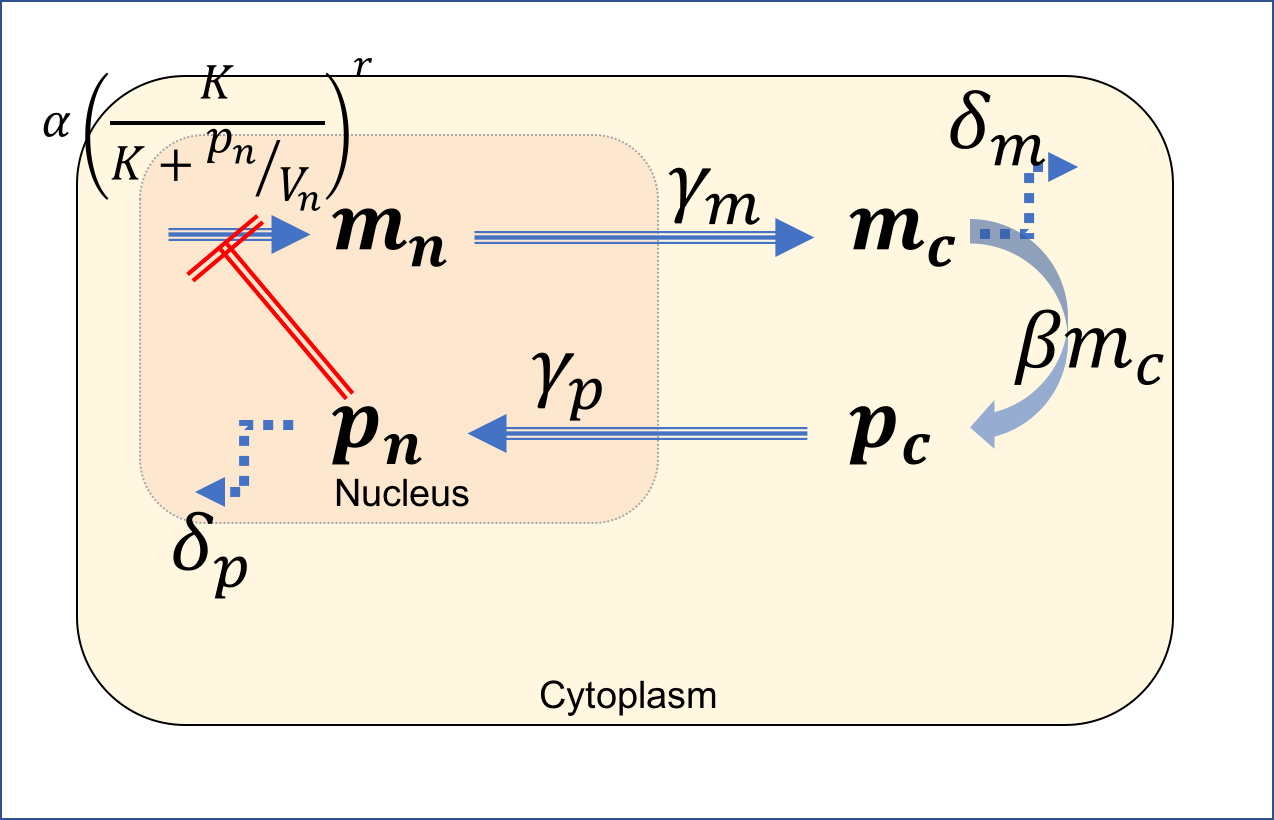
\includegraphics[width=0.5\textwidth]{pathway.png}
	\caption*{\small Figure 1: a schematic cellular clock}
\end {figure}

The variables and parameters that describe the process is the following:
\begin{itemize}
  \item $m_n$: number of mRNAs inside the nucleus;
  \item $m_c$: number of mRNAs in the cytoplasm;
  \item $p_n$: number of protein molecules inside the nucleus;
  \item $p_c$: number of protein molecules in the cytoplasm;
  \item $\alpha$: transcription rate when no proteins are binding;
  \item $\beta$: translation rate from mRNA to protein molecule;
  \item $r$: total number of sites on which the protein can bind;
  \item $K$: the equilibrium constant of the reaction of protein binding to DNA molecules;
  \item $\gamma_m$: the rate at which mRNAs inside the nucleus are transported to cytoplasm;
  \item $\delta_m$: the degradation rate of mRNAs in cytoplasm;
  \item $\gamma_p$: the rate at which the protein molecules in the cytoplasm are transported into nucleus;
  \item $\delta_p$: the degradation rate of this protein inside nucleus;
	\item $V_n$: the volume of the nucleus.
\end{itemize}

Using the above notations, we can define the six reactions involved in the model in Table 1. One remark is that the rate of transcription is $\alpha \{\frac{K}{K + p_n / V_n}\}^r.$ We can think of $\frac{K}{K + p_n / V_n}$ as the possibility that one particular site is not occupied, so it being raised to $r^\text{th}$ power is the probability that all sites are not occupied. The deduction of this expression can be found in Wang and Peskin's work.

\begin{table}[t]
\begin{tabular}{|l|l|l|l|}
\hline
Reaction  & Reaction Name                            & Rate (Probability)                     & Result                                                                         \\ \hline
1          & Transcription of the gene                & $\alpha \{\frac{K}{K + p_n / V_n}\}^r$ & $m_n \to m_n +1$                                                               \\ \hline
2          & Export of mRNA from nucleus to cytoplasm & $\gamma_m m_n$                         & \begin{tabular}[c]{@{}l@{}}$m_n \to m_n -1,$\\ $m_c \to m_c +1$\end{tabular}   \\ \hline
3          & Translation of the mRNA                  & $\beta m_c$                            & $p_c \to p_c + 1$                                                              \\ \hline
4          & Import of protein into nucleus           & $\gamma_p p_c$                         & \begin{tabular}[c]{@{}l@{}}$p_c \to p_c - 1,$\\ $p_n \to p_n + 1$\end{tabular} \\ \hline
5          & Degradation of mRNA in cytoplasm         & $\delta_m m_c$                         & $m_c \to m_c -1$                                                               \\ \hline
6          & Degradation of protein in nucleus        & $\delta_p p_n$                         & $p_n \to p_n -1$                                                               \\ \hline
\end{tabular}
\caption*{\small Table 1: Reaction Table}
\end{table}
The model consists of two versions.
\subsubsection{Deterministic Version}
\hspace{5mm} If we view the number of molecules of each substance as large numbers, the fact that them being integers will have little influence on the model. In this way, we can set up the model using differential equations. Notice that the rate of change of the amount of one substance is equal to the rate that it is produced (imported) minus the rate that it is degraded (exported). This gives us the following:
\begin{equation}
	\frac{dm_n}{dt} = \alpha \{\frac{K}{K + p_n / V_n}\}^r - \delta_m m_n,
\end{equation}

\begin{equation}
	\frac{dm_c}{dt} = \gamma_m m_n - \delta_m m_c,
\end{equation}

\begin{equation}
	\frac{dp_c}{dt} = \beta m_c - \gamma_p p_c,
\end{equation}

\begin{equation}
	\frac{dp_n}{dt} = \gamma_p p_c - \delta_p p_n.
\end{equation}

If we write $k = K V_n,$ then the first equation becomes $\frac{dm_n}{dt} = \alpha \{\frac{k}{k + p_n}\}^r - \delta_m m_n.$ Hence the set of differential equations can also be written as
\begin{equation}
	\frac{dm_n}{dt} = \alpha \{\frac{k}{k + p_n}\}^r - \delta_m m_n,
\end{equation}

\begin{equation}
	\frac{dm_c}{dt} = \gamma_m m_n - \delta_m m_c,
\end{equation}

\begin{equation}
	\frac{dp_c}{dt} = \beta m_c - \gamma_p p_c,
\end{equation}

\begin{equation}
	\frac{dp_n}{dt} = \gamma_p p_c - \delta_p p_n.
\end{equation}

Here we state that, besides modeling, the set of equations can also give insight on the choice of parameters in order to yield an expected oscillation. This is discussed later.


\subsubsection{Stochastic (Microscopic) Version}
\hspace{5mm} On the other hand, we can also look at the microscopic version, keeping track of the number of each molecules when each reaction happens. Recall that if an event has probability per unit time $r$ to happen, and let $T$ denote the time this event first happens, then
\begin{equation}
	\mathbb{P}(T > t) = \lim_{n \to \infty} \prod_{j=1}^{n} (1-\frac{rt}{n}) = \lim_{n \to \infty} (1 - \frac{rt}{n})^n = e^{-rt}.
\end{equation}
So $T$ follows an exponential distribution with parameter $r.$  Since $T$ is continuous, it follows that $F(T),$ the distribution function acting on $T,$ is uniformly distributed on the interval $(0,1).$ Hence, $$-\frac{\log(U)}{r},$$ with $U$ being a random variable uniformly distributed on the interval $(0,1),$ would generate a realization of $T.$

In the stochastic approach, given initial amount of each substances, six reaction times (each follows an exponential distribution with the parameter being the reaction's probability per unit time, respectively) are generated. We assume only the first reaction actually happens. Then the numbers of molecules are adjusted correspondingly and the above process is repeated.

\subsection{Stability Analysis and Choice of Parameters for Single Cell Oscillator Model}
\hspace{5mm} In order to judiciously choose parameters so that the system defined by equations (5)-(8) can sustain a periodic oscillation, we perform a stability analysis of the system. The steady state is defined to be the case when the amount of each substance is not changing with respect to time, i.e. the left hand side of the four equations (5)-(8) are all zeros. This yields
\begin{equation}
	\alpha \{\frac{k}{k + p_n^0}\}^r = \delta_m m_n^0,
\end{equation}

\begin{equation}
    \gamma_m m_n^0 = \delta_m m_c^0,
\end{equation}

\begin{equation}
	\beta m_c^0 = \gamma_p p_c^0,
\end{equation}

\begin{equation}
	\gamma_p p_c^0 = \delta_p p_n^0.
\end{equation}
Here the superscript $0$ denotes the value of the variable in its steady state. Multiplying all the four equations will give us
\begin{equation}
    \alpha \beta \{\frac{k}{k + p_n^0}\}^r = \delta_m \delta_p p_n^0.
\end{equation}
By plotting this we can assure that there is a unique positive steady state, as expected.

Next, we linearize the four equations around the steady state. This gives us

\begin{equation}
    \frac{d\widetilde{m_n}}{dt} = -\eta \widetilde{p_n} - \gamma_m \widetilde{m_n},
\end{equation}
\begin{equation}
	\frac{d \widetilde{m_c}}{dt} = \gamma_m \widetilde{m_n} - \delta_m \widetilde{m_c},
\end{equation}

\begin{equation}
	\frac{d \widetilde{p_c}}{dt} = \beta \widetilde{m_c} - \gamma_p \widetilde{p_c},
\end{equation}

\begin{equation}
	\frac{d \widetilde{p_n}}{dt} = \gamma_p \widetilde{p_c} - \delta_p \widetilde{p_n},
\end{equation}
where
\begin{equation}
    \eta = r \frac{\delta_m \delta_p}{\alpha \beta} \frac{p_n^0}{p_n^0 + k} \alpha,
\end{equation}
 and the variables with tildes are the deviations from the steady state values, e.g. $\widetilde{p_n} = p_n - p_n^0.$ Equations (15)-(18) hold when the deviations are small. A typical case is that after the system reaching equilibrium, there is some small perturbation.

Let $\widetilde{\mathbf{x}} =
\begin{bmatrix}
\widetilde{m_n}  \\
\widetilde{m_c}  \\
\widetilde{p_c}  \\
\widetilde{p_n}
\end{bmatrix}$ and $A =
\begin{bmatrix}
-\gamma_m & 0 & 0 & -\eta \\
\gamma_m &  - \delta_m & 0 & 0 \\
0 &  \beta & - \gamma_p & 0 \\
0 & 0 & \gamma_p &  - \delta_p
\end{bmatrix}.$
It follows that
\begin{equation}
    \frac{d\widetilde{\mathbf{x}}}{dt} = A \widetilde{\mathbf{x}}.
\end{equation} This is a system of ordinary differential equations, and the behaviour of $\widetilde{\mathbf{x}}$ is characterized by the eigenvalues of matrix A. The characteristic equation of matrix A is given by
\begin{align}
    0 &= \det(\lambda I - A) \\
    &= \det \left(\begin{bmatrix}
\lambda + \gamma_m & 0 & 0 & \eta \\
-\gamma_m &  \lambda + \delta_m & 0 & 0 \\
0 &  -\beta & \lambda+\delta_p & 0 \\
0 & 0 & -\gamma_p &  \lambda+ \delta_p
\end{bmatrix}\right) \\
&= (\lambda + \gamma_m)(\lambda + \delta_m)(\lambda + \gamma_p)(\lambda + \delta_p) + \eta \beta \gamma_m \gamma_p \\
&= (\lambda + \gamma_m)(\lambda + \delta_m)(\lambda + \gamma_p)(\lambda + \delta_p) + G \gamma_m \delta_m \gamma_p \delta_p,
\end{align}
where \begin{align}
    G &= \frac{\eta \beta}{\delta_m \delta_p} \\
    &= \left(r \frac{\delta_m \delta_p}{\alpha \beta} \frac{p_n^0}{p_n^0 + k} \alpha\right) \frac{\beta}{\delta_m \delta_p} \\
    &= \left(\frac{p_n^0}{k+p_n^0}\right) r.
\end{align}
The second equality follows from (19).

We claim that the best case for oscillation is that
\begin{equation}
    \gamma_m = \delta_m = \gamma_p = \delta_p = \nu,
\end{equation}
in the sense that they generate oscillation with the smallest $G.$ Proof of this claim can be found in Peskin's work [1]. Now, it follows from (24) that
\begin{align}
    0 &= (\lambda + \nu)^4 + G \nu ^4 \\
    (\lambda + \nu)^4 &= -G \nu ^4 \\
    (\lambda + \nu) &= (-1)^\frac{1}{4} G ^\frac{1}{4}\nu\\
    \lambda &= \mu (-1 + (-1)^\frac{1}{4} G ^\frac{1}{4})
\end{align}
We see that there are four solutions to $\lambda$ and each is a complex number. In order for the system of ODEs (20) to have oscillating solutions, the real part of at least one $\lambda$ must be greater than $0.$ This implies that $G^\frac{1}{4} > \sqrt{2},$ or equivalently, $G>4.$ By (27), \begin{equation}
    \left(\frac{p_n^0}{k+p_n^0}\right) r > 4.
\end{equation}
Since $ \left(\frac{p_n^0}{k+p_n^0}\right) < 1,$ it must be that $r\geq 5.$ Setting $r=5$ and Substituting this into the steady state equation, with some simple algebra we have
\begin{equation}
    \alpha \beta > \nu^2 k \cdot 4(1+4)^5.
\end{equation}
This sheds some light on how the parameters shall be chosen.

\subsection{Multi-Cellular Oscillator}
\hspace{5mm} In this section, we propose three ways of modeling interactions among multiple cells. The simplest approach would be to allow direct diffusion of ``information'' between every two cells. A demonstration of this approach can be seen in Figure 2. \\
\begin {figure}[h]
	\centering
	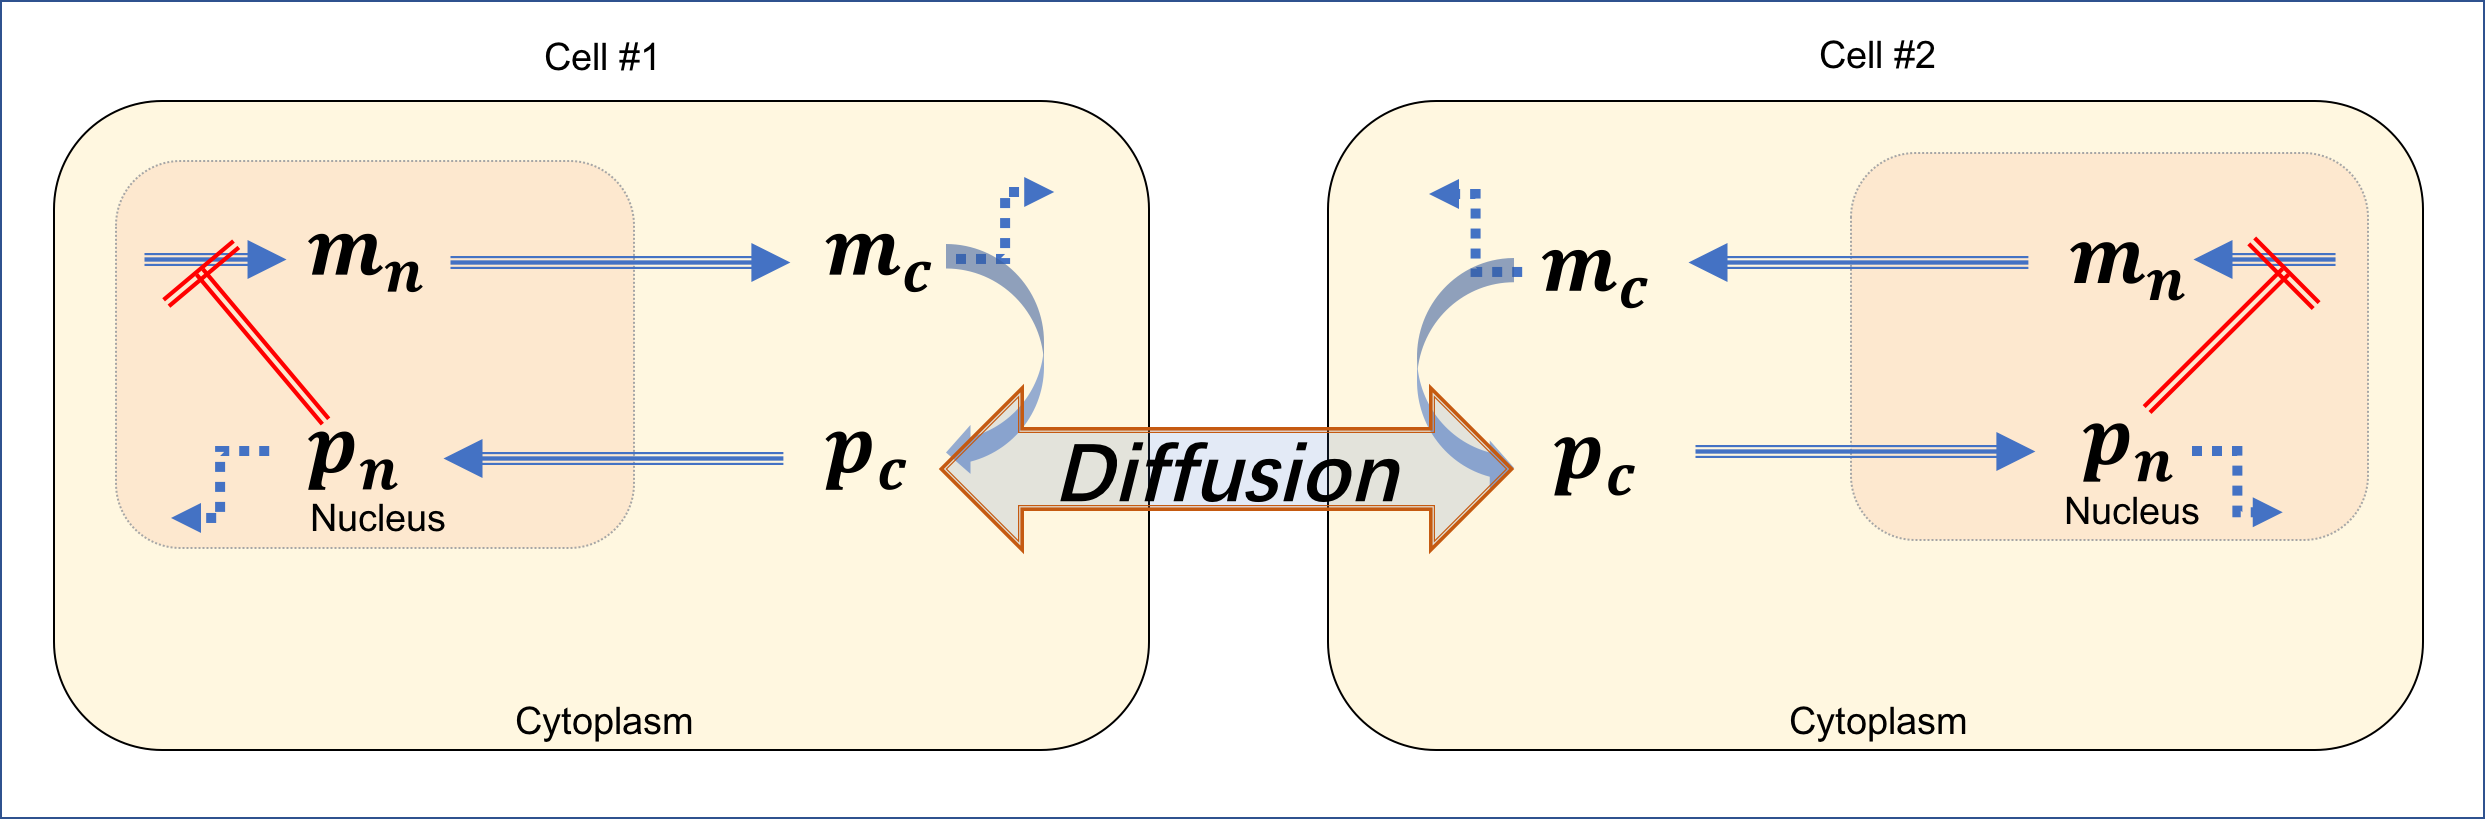
\includegraphics[width=0.7\textwidth]{two_cells.png}
	\caption*{\small Figure 2: Protein diffusion between two cellular oscillators}
\end {figure}

\subsubsection{Direct flow of protein}
\hspace{5mm} This is the easiest version. Assume there is a pipe connecting the two cells and these two cells have the same volume. Protein molecules in one cell can move to the other cell through the pipe. The speed of diffusion is proportional to the difference in the number of protein molecules in the two cells, i.e.
\begin{equation}
	\frac{d {p_c^1}}{dt} = -F ({p_c^1 - p_c^2}),
\end{equation}
\begin{equation}
	\frac{d {p_c^2}}{dt} = -\frac{d {p_c^1}}{dt}.
\end{equation}
Here the superscripts $1$ and $2$ indicate cell 1 and cell 2.

Observe that although this method is simple and concise, it has a limitation that it can only be applied in the case when the two cells are identical in volume. When the volumes are different, it is the concentration, instead of the number of molecules that shall be considered. More importantly, to build a three-cell system we need to build three pipes connecting each of them, and to build a four-cell system we need six pipes. For a system consisting of more than hundreds of cells this method is obviously inefficient and unrealistic. Hence, communicating ``information'' among cells of a multi-cellular organism are usually through a media called extra-cellular fluid rather than a direct diffusion among cells. Some alternative methods are discussed below.

\subsubsection{Direct Diffusion with ECF}
\hspace{5mm} ECF stands for extra-cellular fluid, by which cells live and communicate ``information'' with each other. We consider the case where, instead of connecting two cells with a pipe directly, there are only pipes between each cell and ECF. It means that, every time a protein molecule would like to go from one cell to another, it must go through ECF as a transportation media. \\

Since new entity ECF are considered and we are more concerned with concentration, it would be better to establish some new notations: \\

\textbf{Variables: \\}
\begin{itemize}
    \item $M_n^{(i)}$: concentration of mRNAs inside the nucleus for the ith cell;
    \item $M_c^{(i)}$: concentration of mRNAs in the cytoplasm for the ith cell;
    \item $P_n^{(i)}$: concentration of protein molecules inside nucleus for the ith cell;
    \item $P_c^{(i)}$: concentration of protein molecules in cytoplasm for the ith cell;
    \item $P_{ECF}$: concentration of protein molecules in extra-cellular fluid;
\end{itemize}
\textbf{\hspace{5mm} Parameters: \\}
\begin{itemize}
    \item $\alpha^{(i)}$: transcription rate when no proteins are binding for the ith cell;
    \item $\beta^{(i)}$: translation rate from mRNA to protein molecule for the ith cell;
    \item $r^{(i)}$: total number of sites on which the protein can bind for the ith cell;
    \item $K^{(i)}$: the equilibrium constant of the reaction of protein binding to DNA molecules for the ith cell;
    \item $\gamma_m^{(i)}$: the rate at which mRNAs inside the nucleus are transported to cytoplasm for the ith cell;
    \item $\delta_m^{(i)}$: the degradation rate of mRNAs in cytoplasm for the ith cell;
    \item $\gamma_p^{(i)}$: the rate at which the protein molecules in the cytoplasm are transported into nucleus for the ith cell;
    \item $\delta_p^{(i)}$: the degradation rate of this protein inside nucleus for the ith cell;
    \item $V_n^{(i)}$: volume of the nucleus for the ith cell;
    \item $V_c^{(i)}$: volume of the cytoplasm for the ith cell;
    \item $V_{ECF}$: volume of the ECF;
    \item $\lambda_{ECF}$: the transposition rate at which protein molecules are transported between each cells and ECF;
    \item $n$: number of cells in a given organism.
\end{itemize}

Then, to describe the new dynamical system with ECF as transportation media, we write out a new system of ODE's:\\

\begin{align}
    \frac{dM_n^{(i)}}{dt} &= \frac{\alpha^{(i)}}{V_n^{(i)}} \{\frac{K^{(i)}}{K^{(i)} + P_n^{(i)}}\}^{r^{(i)}} - \gamma_m^{(i)} M_n^{(i)} \\
    \frac{dM_c^{(i)}}{dt} &= \gamma_m^{(i)} (\frac{V_n^{(i)}}{V_c^{(i)}}) M_n^{(i)} - \delta_m^{(i)} M_c^{(i)} \\
    \frac{dP_c^{(i)}}{dt} &= \beta^{(i)} M_c^{(i)} - \gamma_p^{(i)} P_c^{(i)} - \lambda_{ECF} (P_c^{(i)} - P_{ECF})\\
    \frac{dP_n^{(i)}}{dt} &= \gamma_p^{(i)} (\frac{V_c^{(i)}}{V_n^{(i)}}) P_c^{(i)} - \delta_p^{(i)} P_n^{(i)} \\
    \frac{dP_{ECF}}{dt} &= \sum_i^n \lambda_{ECF} \frac{V_c^{(i)}}{V_{ECF}} (P_c^{(i)} - P_{ECF})
\end{align}

\vspace{15mm}

\textbf{Stability Analysis}
With the dynamical system described above, we do analysis on stability of this system by analyzing eigenvalues of the linearized ODE system around steady state. Denote $M_n^{(i)0}, M_c^{(i)0}, P_c^{(i)0}, P_c^{(i)0}, P_{ECF}^{(i)0}$, for $i \in \{1, ..., n\}$, as the value for variables at a steady state. Then, as before, denote $\widetilde{M_n^{(i)}} = M_n^{(i)} - M_n^{(i)0}$, $\widetilde{P_n^{(i)}} = P_n^{(i)} - P_n^{(i)0}$, and etc.. Therefore, we have a system of linearized equation around steady state:

\begin{align}
    \frac{d\widetilde{M_n^{(i)}}}{dt} &= a^{(i)} \widetilde{P_n^{(i)}} - \gamma_m^{(i)} \widetilde{M_n^{(i)}}, \\
    \frac{d\widetilde{M_c^{(i)}}}{dt} &= \gamma_m^{(i)} (\frac{V_n^{(i)}}{V_c^{(i)}}) \widetilde{M_n^{(i)}} - \delta_m^{(i)} \widetilde{M_c^{(i)}}, \\
    \frac{d\widetilde{P_c^{(i)}}}{dt} &= \beta^{(i)} \widetilde{M_c^{(i)}} - (\gamma_p^{(i)} + \lambda_{ECF}) \widetilde{P_c^{(i)}} + \lambda_{ECF} \widetilde{P_{ECF}} \\
    \frac{d\widetilde{P_n^{(i)}}}{dt} &= \gamma_p^{(i)} (\frac{V_c^{(i)}}{V_n^{(i)}}) \widetilde{P_c^{(i)}} - \delta_p^{(i)} \widetilde{P_n^{(i)}}, \\
    \frac{d\widetilde{P_{ECF}}}{dt} &= \sum_i^n \lambda_{ECF} \frac{V_c^{(i)}}{V_{ECF}} \widetilde{P_c^{(i)}} - n \lambda_{ECF} \frac{V_c^{(i)}}{V_{ECF}} \widetilde{P_{ECF}},
\end{align}

where $a^{(i)} = -\frac{\alpha^{(i)} r^{(i)}}{V_n^{(i)} K^{(i)}} \{\frac{K^{(i)}}{K^{(i)} + P_n^{(i)0}}\}^{r^{(i)} + 1}$. \\

At this point, in order to simplify this dynamical system for the sake of stability analysis and, meanwhile, to keep interesting features of the system, we do the followings: \\
\begin{itemize}
    \item Let n = 2, and
    \item let $\gamma_m^{(i)} = \gamma_p^{(i)} = \delta_m^{(i)} = \delta_p^{(i)} = \lambda^{(i)}$ for $i \in \{1, 2\}$.
\end{itemize}
Thus, this linear system could also be rewritten as $\Dot{X} = AX$, where $A =$
\begin{center}

$
\begin{bmatrix}
-\lambda^{(1)}                  & 0             & 0                             & a^{(1)}                       &0           &0                               &0               &0                          &0                                  \\

\lambda^{(1)} \frac{V_c^{(1)}}{V_n^{(1)}}& - \lambda^{(1)}   & 0                             & 0                         &0           &0                               &0               &0                          &0                                  \\

0                           & \beta^{(1)}       & - (\lambda^{(1)} + \lambda_{ECF}) & 0                         &0           &0                               &0               &0                          &\lambda_{ECF} \\

0                           & 0             & \lambda^{(1)} \frac{V_n^{(1)}}{V_c^{(1)}} & - \lambda^{(1)}               &0           &0                               &0               &0                          &0                                  \\
%%%%%%%%%%%%%%%%%%%%%%%%%%%%%%%%%%%%%%%%%%%%%%%%%%%%%%%%%%%%%%%%%%%%%%%%%%%%%%%%%%%%%%%%%%%%%%%%%%%%%%%%%%%%%%%%%%%%%%%%%%%%%%%%%%%%%%%%%%%%%%%%%%%%%%%%%%%%%%%%%%%
0 & 0 & 0 & 0 & -\lambda^{(2)}                      &0              & 0                                 & a^{(2)}                                  &0  \\

0 & 0 & 0 & 0 & \lambda^{(2)}\frac{V_c^{(2)}}{V_n^{(2)}}    & -\lambda^{(2)}    & 0                                 & 0                                     &0  \\

0 & 0 & 0 & 0 & 0                               & \beta^{(2)}       & -(\lambda^{(2)} + \lambda_{ECF})      & 0                         &\lambda_{ECF}\\

0 & 0 & 0 & 0 & 0                               & 0             & \lambda^{(2)} \frac{V_n^{(2)}}{V_c^{(2)}}     & -\lambda^{(2)}
&0 \\

0 & 0 & \lambda_{ECF} \frac{V_c^{(1)}}{V_{ECF}} & 0 & 0                               & 0             & \lambda_{ECF} \frac{V_c^{(2)}}{V_{ECF}}     & 0
&- \sum_{i=1}^{2} \{\lambda_{ECF} \frac{V_c^{(i)}}{V_{ECF}}\}\\

\end{bmatrix}$

\end{center}

, $X^T =
\begin{bmatrix}
\widetilde{M_n^{(1)}} &
\widetilde{M_c^{(1)}} &
\widetilde{P_c^{(1)}} &
\widetilde{P_n^{(1)}} &
\widetilde{M_n^{(2)}} &
\widetilde{M_c^{(2)}} &
\widetilde{P_c^{(2)}} &
\widetilde{P_n^{(2)}} &
\widetilde{P_{ECF}}
\end{bmatrix}$, and $\Dot{X} = \frac{dX}{dt}$. \\

To express matrix $A$ explicitly in terms of parameters, we solve for $P_n^{(1)0}$ and $P_n^{(2)0}$ and thus we could get $a^{(1)}$ and $a^{(2)}$. \\


With \textit{MatLab}, we could compute all eigenvalues of A and store them in $E = \{e_j\}_{j \in \{1, ...,9\}}$, where $e_j \in \mathbb{C}$. Let $e_{max} = argmax_{\{e_j \in E\}} \{real(e_j)\}$, then if $real(e_{max}) > 0$, this system around the steady state is unstable. Otherwise, we could conclude that the system around such a steady state is stable. \\


\textbf{Synchronization} We will show by empirical results that the periods of oscillation of two and more cells are influenced by communications among them as well as ECF. Moreover, we will also verify that there are some cases where a tendency to a synchronized period among cells could be observed. \\


\textbf{Limitations}
Some limitations of this model may be, in most case, protein transportation does not happen only based on concentration differences between two sides of cell membrane. In other words, this process is usually not a passive free diffusion but very often a active transport, which involves control from cells based on concentration of protein. \\

In light of this, we propose the next model -- \textit{Positive Feedback Transposition with ECF}.

\subsubsection{Positive Feedback Transposition with ECF}
\hspace{5mm} Considering the process of transporting protein from side $A$ of cell membrane to the other side $B$. And, there are $r$ binding sites for this protein on the face of membrane on side $A$. With more sites been occupied, the speed of transportation increases, i.e. positive feedback. We could assume the binding and unbinding reactions are in rapid equilibrium with equilibrium constant $K$. Also, the transportation rate with no binding sites been occupied is $\alpha$.

\begin{figure} [h]
    \centering
	\begin{minipage}{0.45\textwidth}
		\centering
		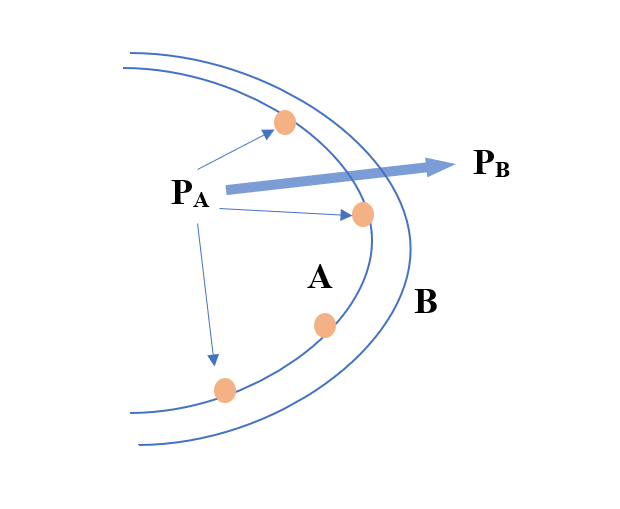
\includegraphics[width=0.89\textwidth]{PFAn.png}
		\caption*{\small Figure X: Animation of PFT}
	\end{minipage}

\end{figure}


To formalize this idea, we need to introduce more parameters in order to describe this dynamical system. \\

\textbf{\hspace{5mm}More Parameters: \\}
\begin{itemize}
    \item $\alpha_{ex}^{(i)}$: exporting rate when no proteins are binding on the inner side of cell membrane for the ith cell;
    \item $\alpha_{im}^{(i)}$: importing rate when no proteins are binding on the outer side of cell membrane for the ith cell;
    \item $r_{ex}^{(i)}$: total number of sites on the inner side of cell membrane on which the protein can bind in the ith cell;
    \item $r_{im}^{(i)}$: total number of sites on the outer side of cell membrane on which the protein can bind for the ith cell;
    \item $K_{ex}^{(i)}$: the equilibrium constant of the reaction of protein binding to sites on the inner face of cell membrane for the ith cell;
    \item $K_{im}^{(i)}$: the equilibrium constant of the reaction of protein binding to sites on the outer face of cell membrane for the ith cell.
\end{itemize}

\begin{align}
    \frac{dM_n^{(i)}}{dt} &= \frac{\alpha^{(i)}}{V_n^{(i)}} \{\frac{K^{(i)}}{K^{(i)} + P_n^{(i)}}\}^{r^{(i)}} - \gamma_m^{(i)} M_n^{(i)} \\
    \frac{dM_c^{(i)}}{dt} &= \gamma_m^{(i)} (\frac{V_n^{(i)}}{V_c^{(i)}}) M_n^{(i)} - \delta_m^{(i)} M_c^{(i)} \\
    \frac{dP_c^{(i)}}{dt} &= \beta^{(i)} M_c^{(i)} - \gamma_p^{(i)} P_c^{(i)} - \frac{\alpha_{ex}^{(i)}}{V_c^{(i)}} (\frac{P_c^{(i)}}{K_{ex}^{(i)} + P_c^{(i)}})^{r_{ex}^{(i)}} + \frac{\alpha_{im}^{(i)}}{V_c^{(i)}} (\frac{P_{ECF}}{K_{im}^{(i)} + P_{ECF}})^{r_{im}^{(i)}} \\
    \frac{dP_n^{(i)}}{dt} &= \gamma_p^{(i)} (\frac{V_c^{(i)}}{V_n^{(i)}}) P_c^{(i)} - \delta_p^{(i)} P_n^{(i)} \\
    \frac{dP_{ECF}}{dt} &= \sum_i^n (\frac{\alpha_{ex}^{(i)}}{V_{ECF}} (\frac{P_c^{(i)}}{K_{ex}^{(i)} + P_c^{(i)}})^{r_{ex}^{(i)}} - \frac{\alpha_{im}^{(i)}}{V_{ECF}} (\frac{P_{ECF}}{K_{im}^{(i)} + P_{ECF}})^{r_{im}^{(i)}})
\end{align}

\newpage

\section{Results}
\subsection{A Single Cellular Oscillator}
\hspace{5mm} Throughout the section we will use the amount of $m_n$, mRNAs in nucleus, to draw results and conclusions about circadian oscillations.

We first show the results of one cellular oscillator. The parameters are chosen as following: $r = 5,$ $k= 200,$ $\alpha = 100000,$ $\beta = 10,$ $\nu = \gamma_m = \gamma_p = \delta_m =\delta_p = 0.285599.$ Here $\nu$ is chosen to be $0.285599$ as this would give an oscillator whose period is close to 24 hours. $r$ is chosen to be the smallest possible value that allows the model to work. $\alpha, \beta$ and $k$ are chosen as such that realistic case is mimicked and equation (34) holds. Initial values of $p_n, p_c, m_n$ and $m_c$ do not play an critical role in the oscillation. In fact, as long as the initial values are not set to extremely large or small numbers, given sufficiently long time, the system will settle itself down and converge to a periodic oscillation, with $p_n, p_c, m_n$ and $m_c$ each fluctuating around roughly $1200, 1200, 40$ and $35,$ respectively. For example, a graph plotting the number of molecules of each substance, with the initial state set to $p_n = 500, p_c = 500, m_n = 500$ and $m_c = 500$, is shown in Figure X.
\begin{figure}[h]
    \centering
	\begin{minipage}{0.5\textwidth}
		\centering
		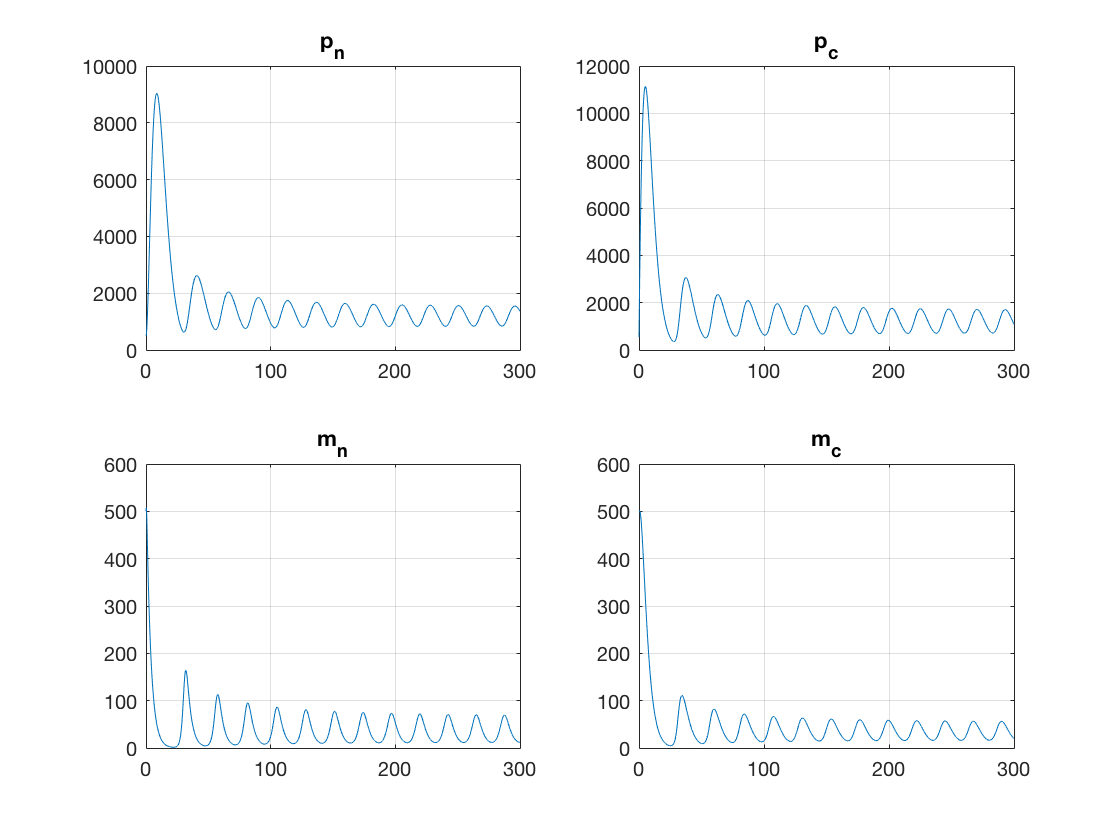
\includegraphics[width=0.99\textwidth]{single_cell_show_convergence.png}
		\caption*{\small Figure X: Convergence to oscillation ultimately.}
	\end{minipage}

\end{figure}

It can be seen that after about 150 hours of reaction, the system converges to the periodic oscillation as specified above. We manually set the four initial values to be $p_n = 925, p_c = 730,m_n = 32$ and $m_c = 21$ at $t=0.$ We denote this set of values as the initial state for the oscillator. This set of values is (approximately) taken at some time when the system has already started its regular oscillation, so that our model will not go through the transition to regular oscillation. In fact, for purpose of comparison, this is the state in which $p_c$ starts at its lowest value.

\begin{figure}[h]
    \centering
	\begin{minipage}{0.45\textwidth}
		\centering
		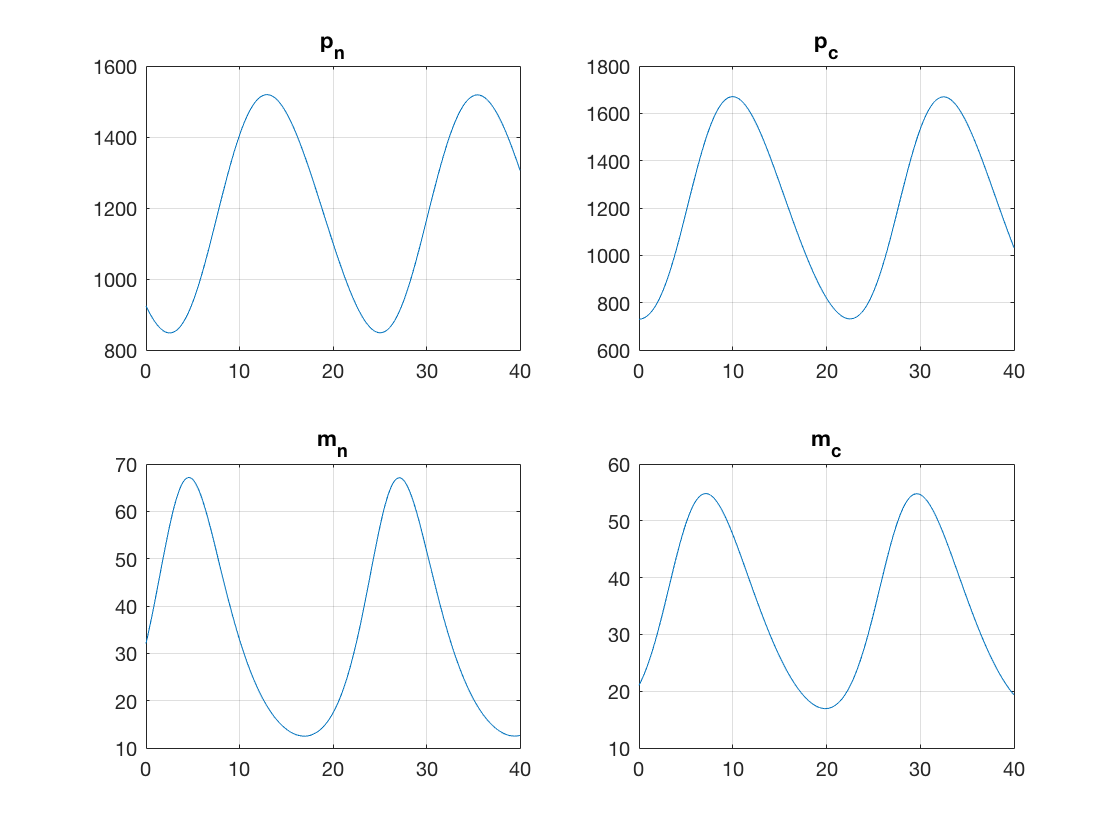
\includegraphics[width=0.89\textwidth]{single_oscillator_zoom_in.png}
		\caption*{\small Figure X: Deterministic version, up to $t=40.$}
	\end{minipage}
	\begin{minipage}{0.45\textwidth}
		\centering
		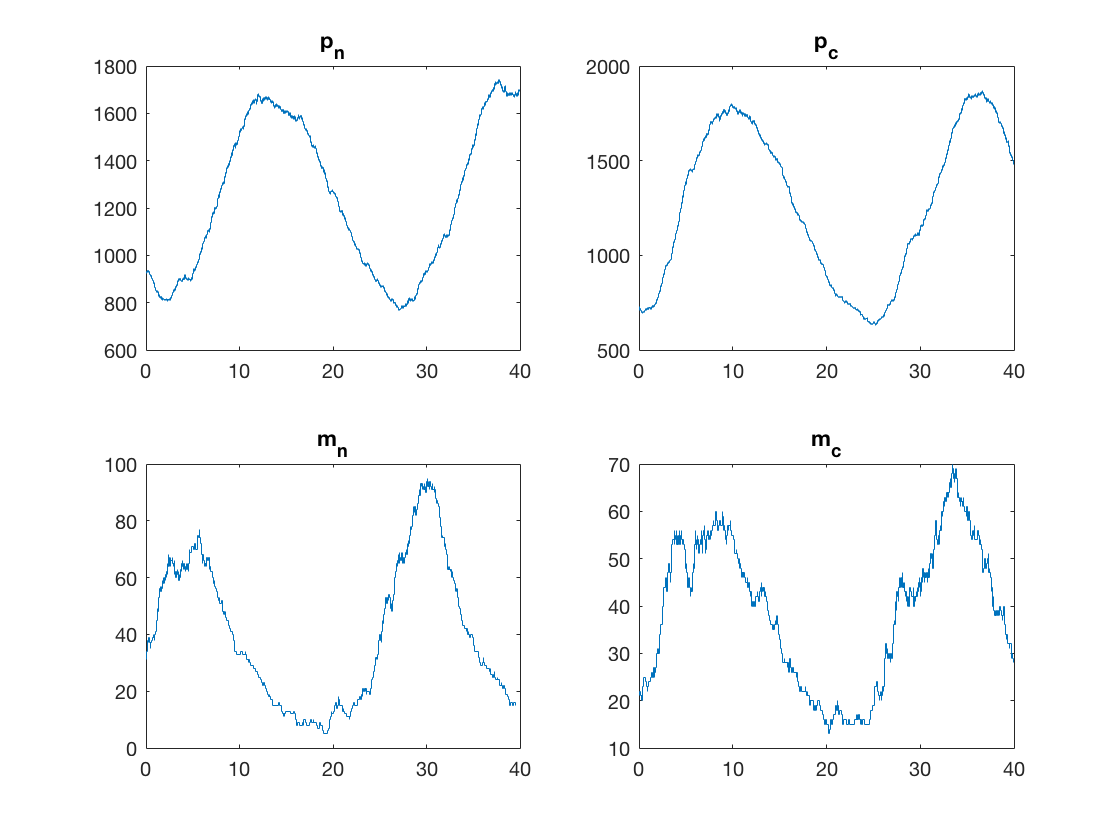
\includegraphics[width=0.89\textwidth]{sto_single_oscillator_zoom_in.png}
		\caption*{\small Figure X: Stochastic version, up to $t=40.$}
	\end{minipage}
	\begin{minipage}{0.45\textwidth}
		\centering
		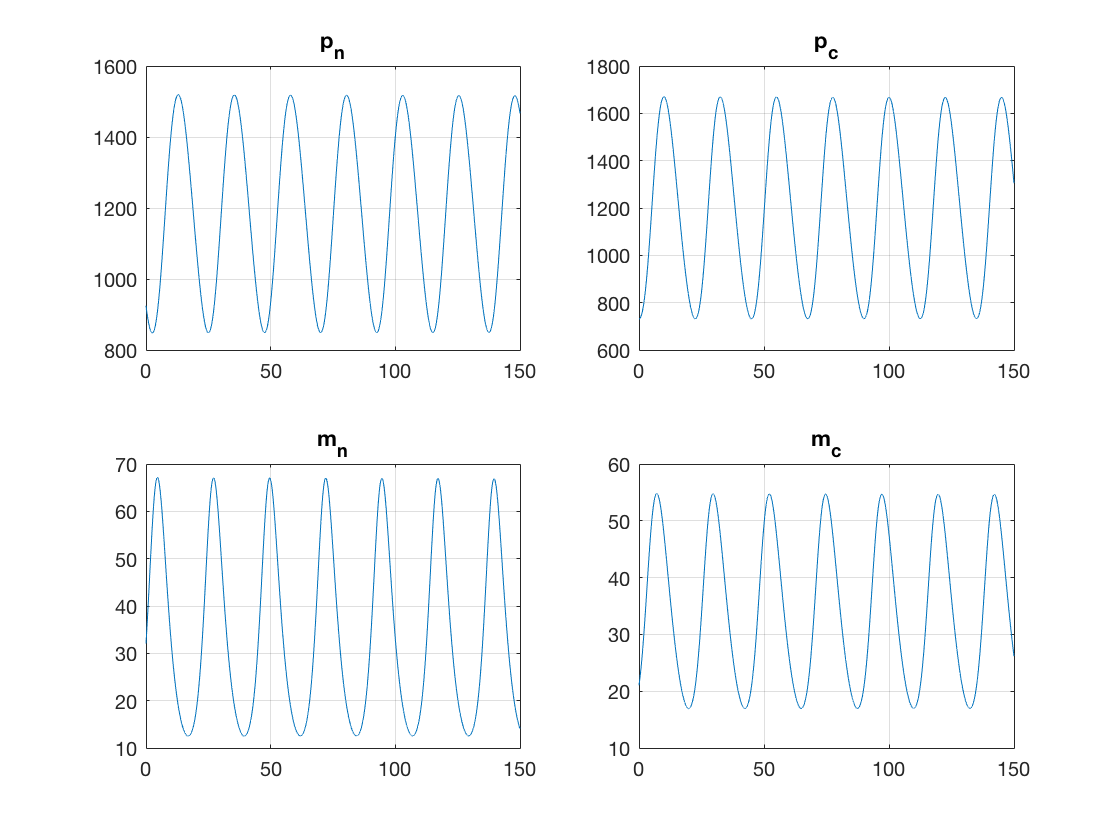
\includegraphics[width=0.89\textwidth]{single_oscillator_zoom_out.png}
		\caption*{\small Figure X: Deterministic version, up to $t=150.$}
	\end{minipage}
	\begin{minipage}{0.45\textwidth}
		\centering
		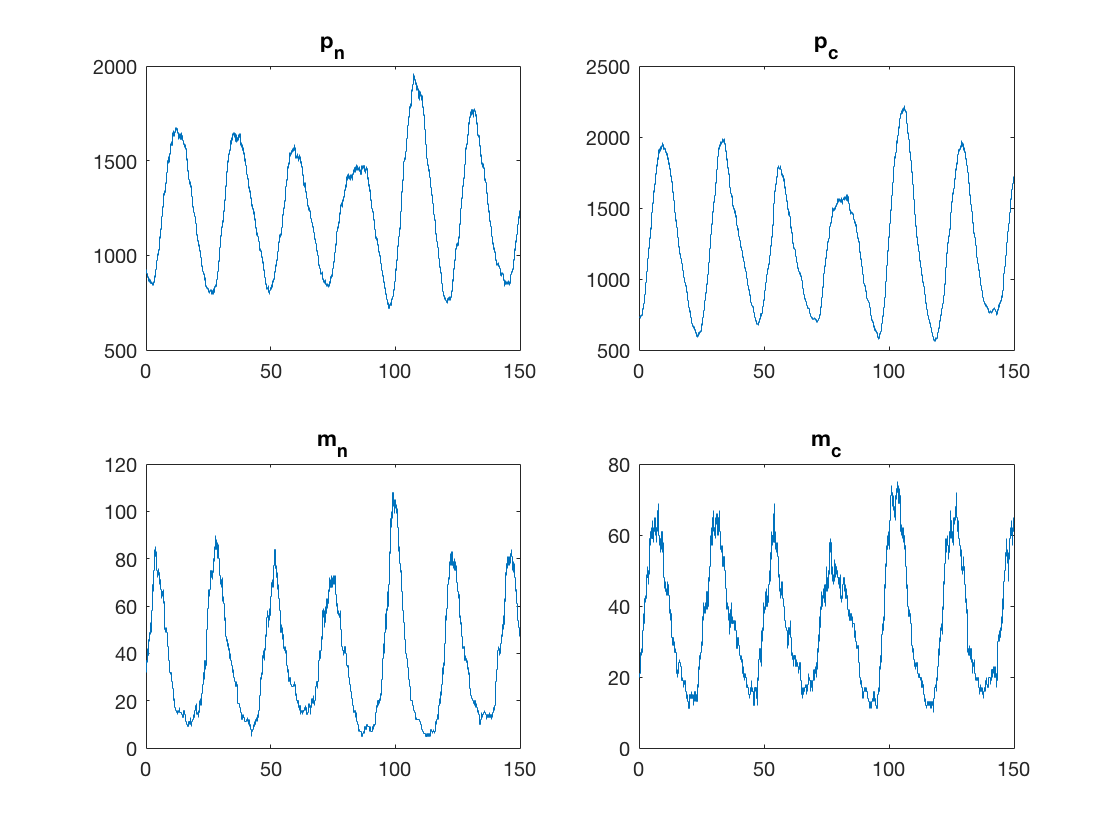
\includegraphics[width=0.89\textwidth]{sto_single_oscillator_zoom_out.png}
		\caption*{\small Figure X: Stochastic version, up to $t=150.$}
	\end{minipage}

\end{figure}

Using the above specification, two types of simulation, the deterministic version as well as the stochastic version, are both implemented. As mentioned above, the deterministic version is described by equations (5)-(8). The stochastic version is described by the last column in Table 1. A code snippet is shown below.

\begin{lstlisting}
    [Tmin, kmin] = min(T);
    % Tmin is the time it takes for the "happened" reaction to happen.
    % kmin is the position (1,2,3,4,5,6) indicating which reaction happens
    switch kmin
        case 1
            % transcription happens
            m_n = m_n + 1;
        case 2
            % mRNA enters cytoplasm from nucleus
            m_n = m_n - 1;
            m_c = m_c + 1;
        case 3
            % translation happens
            p_c = p_c + 1;
        case 4
            % protein enters nucleus from cytoplasm
            p_c = p_c - 1;
            p_n = p_n + 1;
        case 5
            % degradation of mRNA
            m_c = m_c - 1;
        case 6
            % degradation of protein
            p_n = p_n - 1;
    end
    t = t + Tmin;
\end{lstlisting}



\begin{figure}[!]
    \centering
	\begin{minipage}{0.99\textwidth}
		\centering
		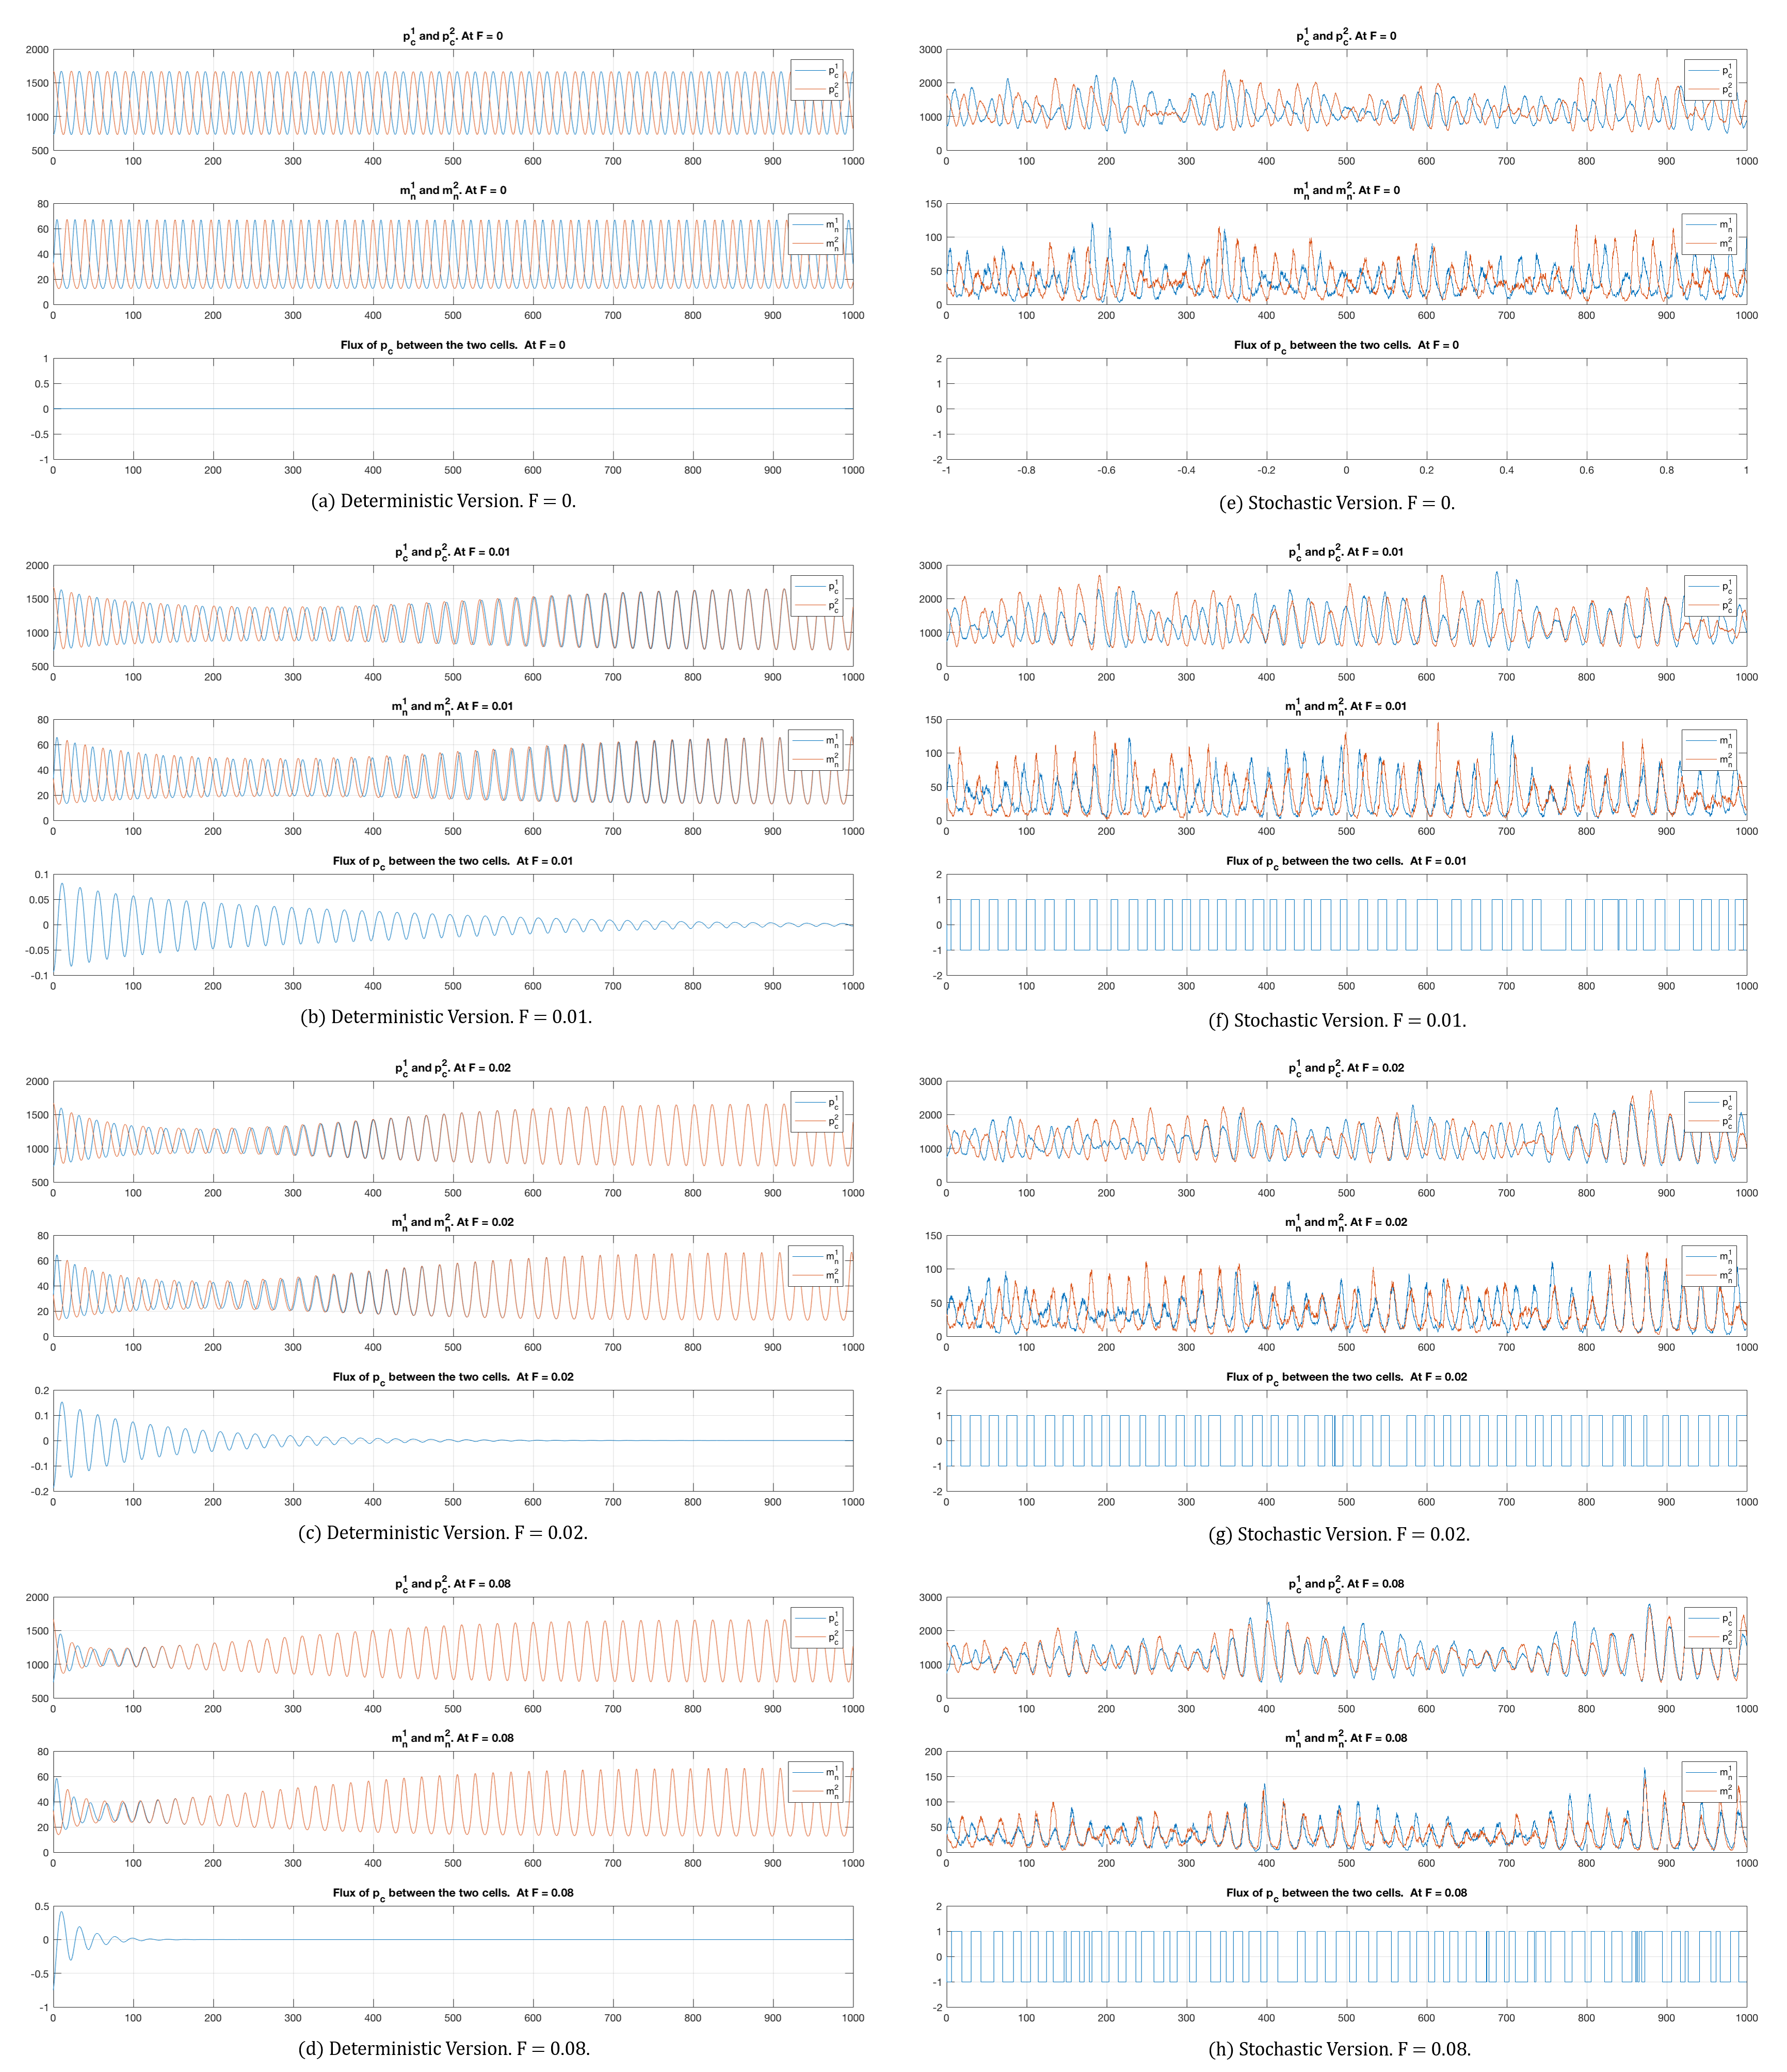
\includegraphics[width=0.99\textwidth]{combined_results.png}
		\caption*{\small Figure X. Two identical cells with different initial states.}
	\end{minipage}
	\footnotesize
	\emph{Graphs on the left column are deterministic versions. Graphs on the right column are stochastic versions. Graphs on the same row are plotted for models with the same value of $F.$ The first and second plot in each graph are the number of proteins in cytoplasm and mRNAs in nucleus. The third plot is the flow of protein. Observe that each two graphs in the same row look similar.}
\end{figure}

Results from both versions are plotted in Figure X. The numbers of molecules of each substance are plotted in each figure. (a)-(d) are deterministic version, whose reaction times are set to 40 hours and 150 hours, respectively. Figure (e)-(h) are stochastic version, which are stair-case functions, whose reaction times are set to 40 hours and 150 hours, respectively. Observe that the results from the stochastic version resemble those from the deterministic version. Both versions show an oscillating period of about 24 hours. This confirms our expectation.


\subsection{Two cellular oscillators with direct flow of protein}
\subsubsection{Two cells with only phase difference}
\hspace{5mm} We use the direct flow of protein molecules, described in equations (35) and (36), to examine how two cells can synchronize their oscillations. Consider two identical cells, each of which has a circadian oscillation discussed above, whose only difference is the initial state. We manually set the initial state of the first cell to be $p^1_n = 925, p^1_c = 730, m^1_n = 32$ and $m^1_c = 21,$ and the initial state of the second cell to be $p^2_n = 1403, p^2_c = 1670, m^2_n = 33$ and $m^2_c = 48.$ These values are chosen such at both cells fall in regular oscillating cycles, and that $p^1_c$ starts at its nadir and $p^2_c$ starts at its zenith. Equivalently, the two oscillations in the two cells have a phase difference of $\frac{1}{2}T,$ with $T$ being the common period.

Imagine that the two cells are connected by a pipe and there is a valve, represented by the value of $F$ in our model. If the valve is shut down, or $F=0,$ then obviously there is no flow of protein between the two cells. The two cells would each follow its individual circadian rhythm, so the phase difference of $\frac{1}{2}T$ would be eternally kept, regardless of how long the reactions have happened. This is demonstrated in Figure X(a). Observe that the flow of protein is constantly zero and the oscillations in each cell are not interacting at all with each other.


Next we open the valve a little bit, by setting $F = 0.01.$ $p_c$ and $m_n$ in each cell, and the flow protein across time are plotted in Figure X(b). We can see that although the phase difference is large at the beginning, the flow of protein drags the two oscillations together so that in approximately 100 hours, the phase difference almost gets eliminated and the two cells run on a shared, synchronized circadian rhythm. Also notice that the flow of protein gradually damps down as the two oscillations gradually converge.


It is natural to expect that, if faster flow is allowed, the convergence would also be faster. Results from modeling with $F = 0.02$ and $F=0.08$ are plotted in Figure X(c) and (d), and they confirm our expectation. When $F$ is set to be $0.02,$ after about 500 hours of synchronization, the phase difference becomes indiscernible. When $F$ is set to be $0.08,$ we can see that the synchronization becomes much faster. It only takes about 100 hours for the two cells to synchronize their oscillations. Also notice that the magnitude of the flow of proteins during synchronization is much larger than that in previous cases.

The corresponding stochastic versions are plotted in Figure X(e), (f), (g) and (h). Results are similar in the sense that $F=0$ yields no convergence, while $F = 0.01, 0.02, 0.08$ each yield successful synchronization of the two circadian oscillation, with consecutively faster and faster rate of convergence. Comparing (b) and (f), and (c) and (g), we suspect that perhaps in the stochastic model, the shorter amount of time, as the inherent noise in the stochastic system may actually help the synchronization. Nevertheless, due to its stochastic nature, we cannot prove this conjecture without further research.

In the case where two cells have identical structure, but only phase difference, we conclude that the synchronization is easy. With some protein flow, the two systems can align themselves to a shared oscillation. This resembles the information exchange in cells in the same organ, as they tend to have almost the same structure, but their being born at different time generate the phase differences among them. The result is not surprising, but what is remarkable is that, some very slight amount of protein flow between the two cells (i.e. $F$ is very small) would be sufficient to allow the two cells to get synchronized.

\subsubsection{Two cells with different oscillating periods}

\begin{figure}[h]
    \centering
	\begin{minipage}{0.99\textwidth}
		\centering
		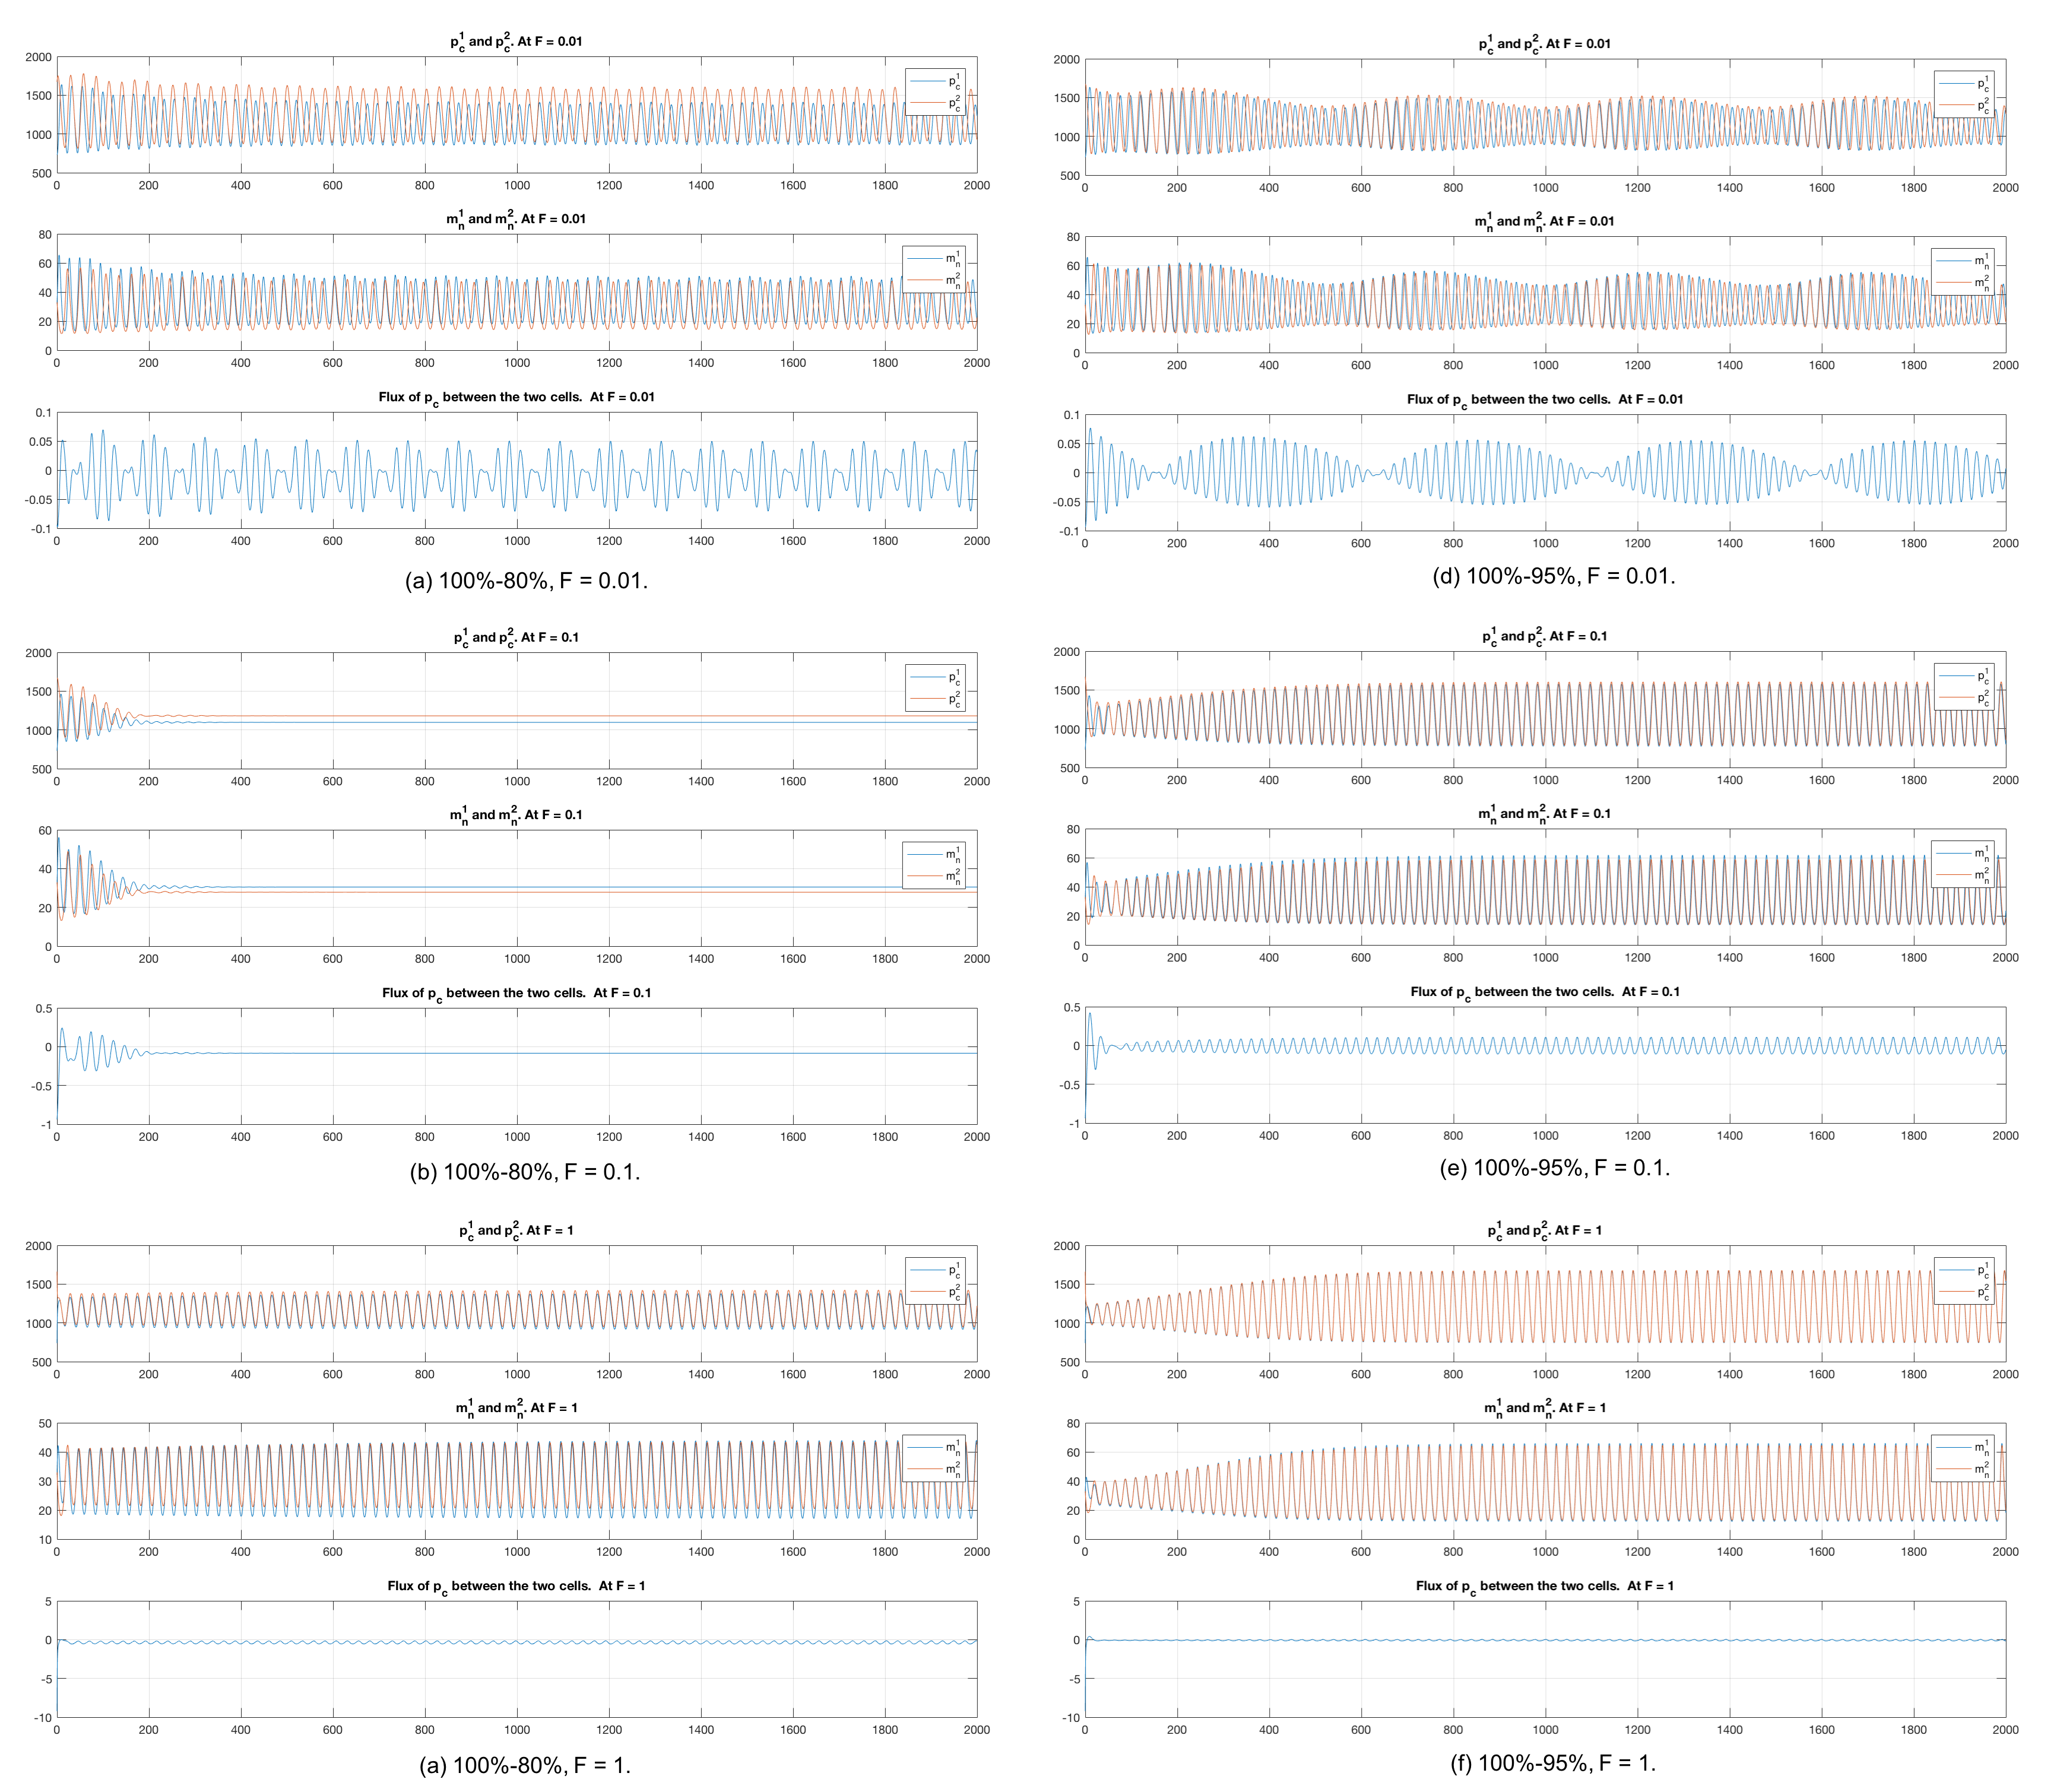
\includegraphics[width=0.99\textwidth]{diff_periods_combine.png}
		\caption*{\small Figure X.}
	\end{minipage}
	\footnotesize
	\emph{Graphs in the left column are plotted for the cases when the period of cell 2 is approximately 80\% of that of cell 1, and graphs in the right column are plotted for the cases when the period of cell 2 is approximately 95\% of that of cell 1. Graphs in the same row are plotted for cases with the same value of $F$. The first and second plot in each graph are the number of proteins in cytoplasm and mRNAs in nucleus. The third plot is the flow of protein. All are deterministic versions.}
\end{figure}

 Using the same method, we also study the case where two cells have different oscillating periods. The assumption is the following: the two cells are still identical, but they are put in different environment (e.g. there may be difference in temperature, pH, etc.). The influence is that the same pathway is processed at different rates in the two cells. Hence, the two cells have innately different circadian rhythms. To simply the setting, we fix one cell, as described above, and perturb the parameters of the other cell by some factor. We study how the flow of protein between the two cells can potentially synchronize the two innately different periods.

 \begin{figure}[!]
    \centering
	\begin{minipage}{0.99\textwidth}
		\centering
		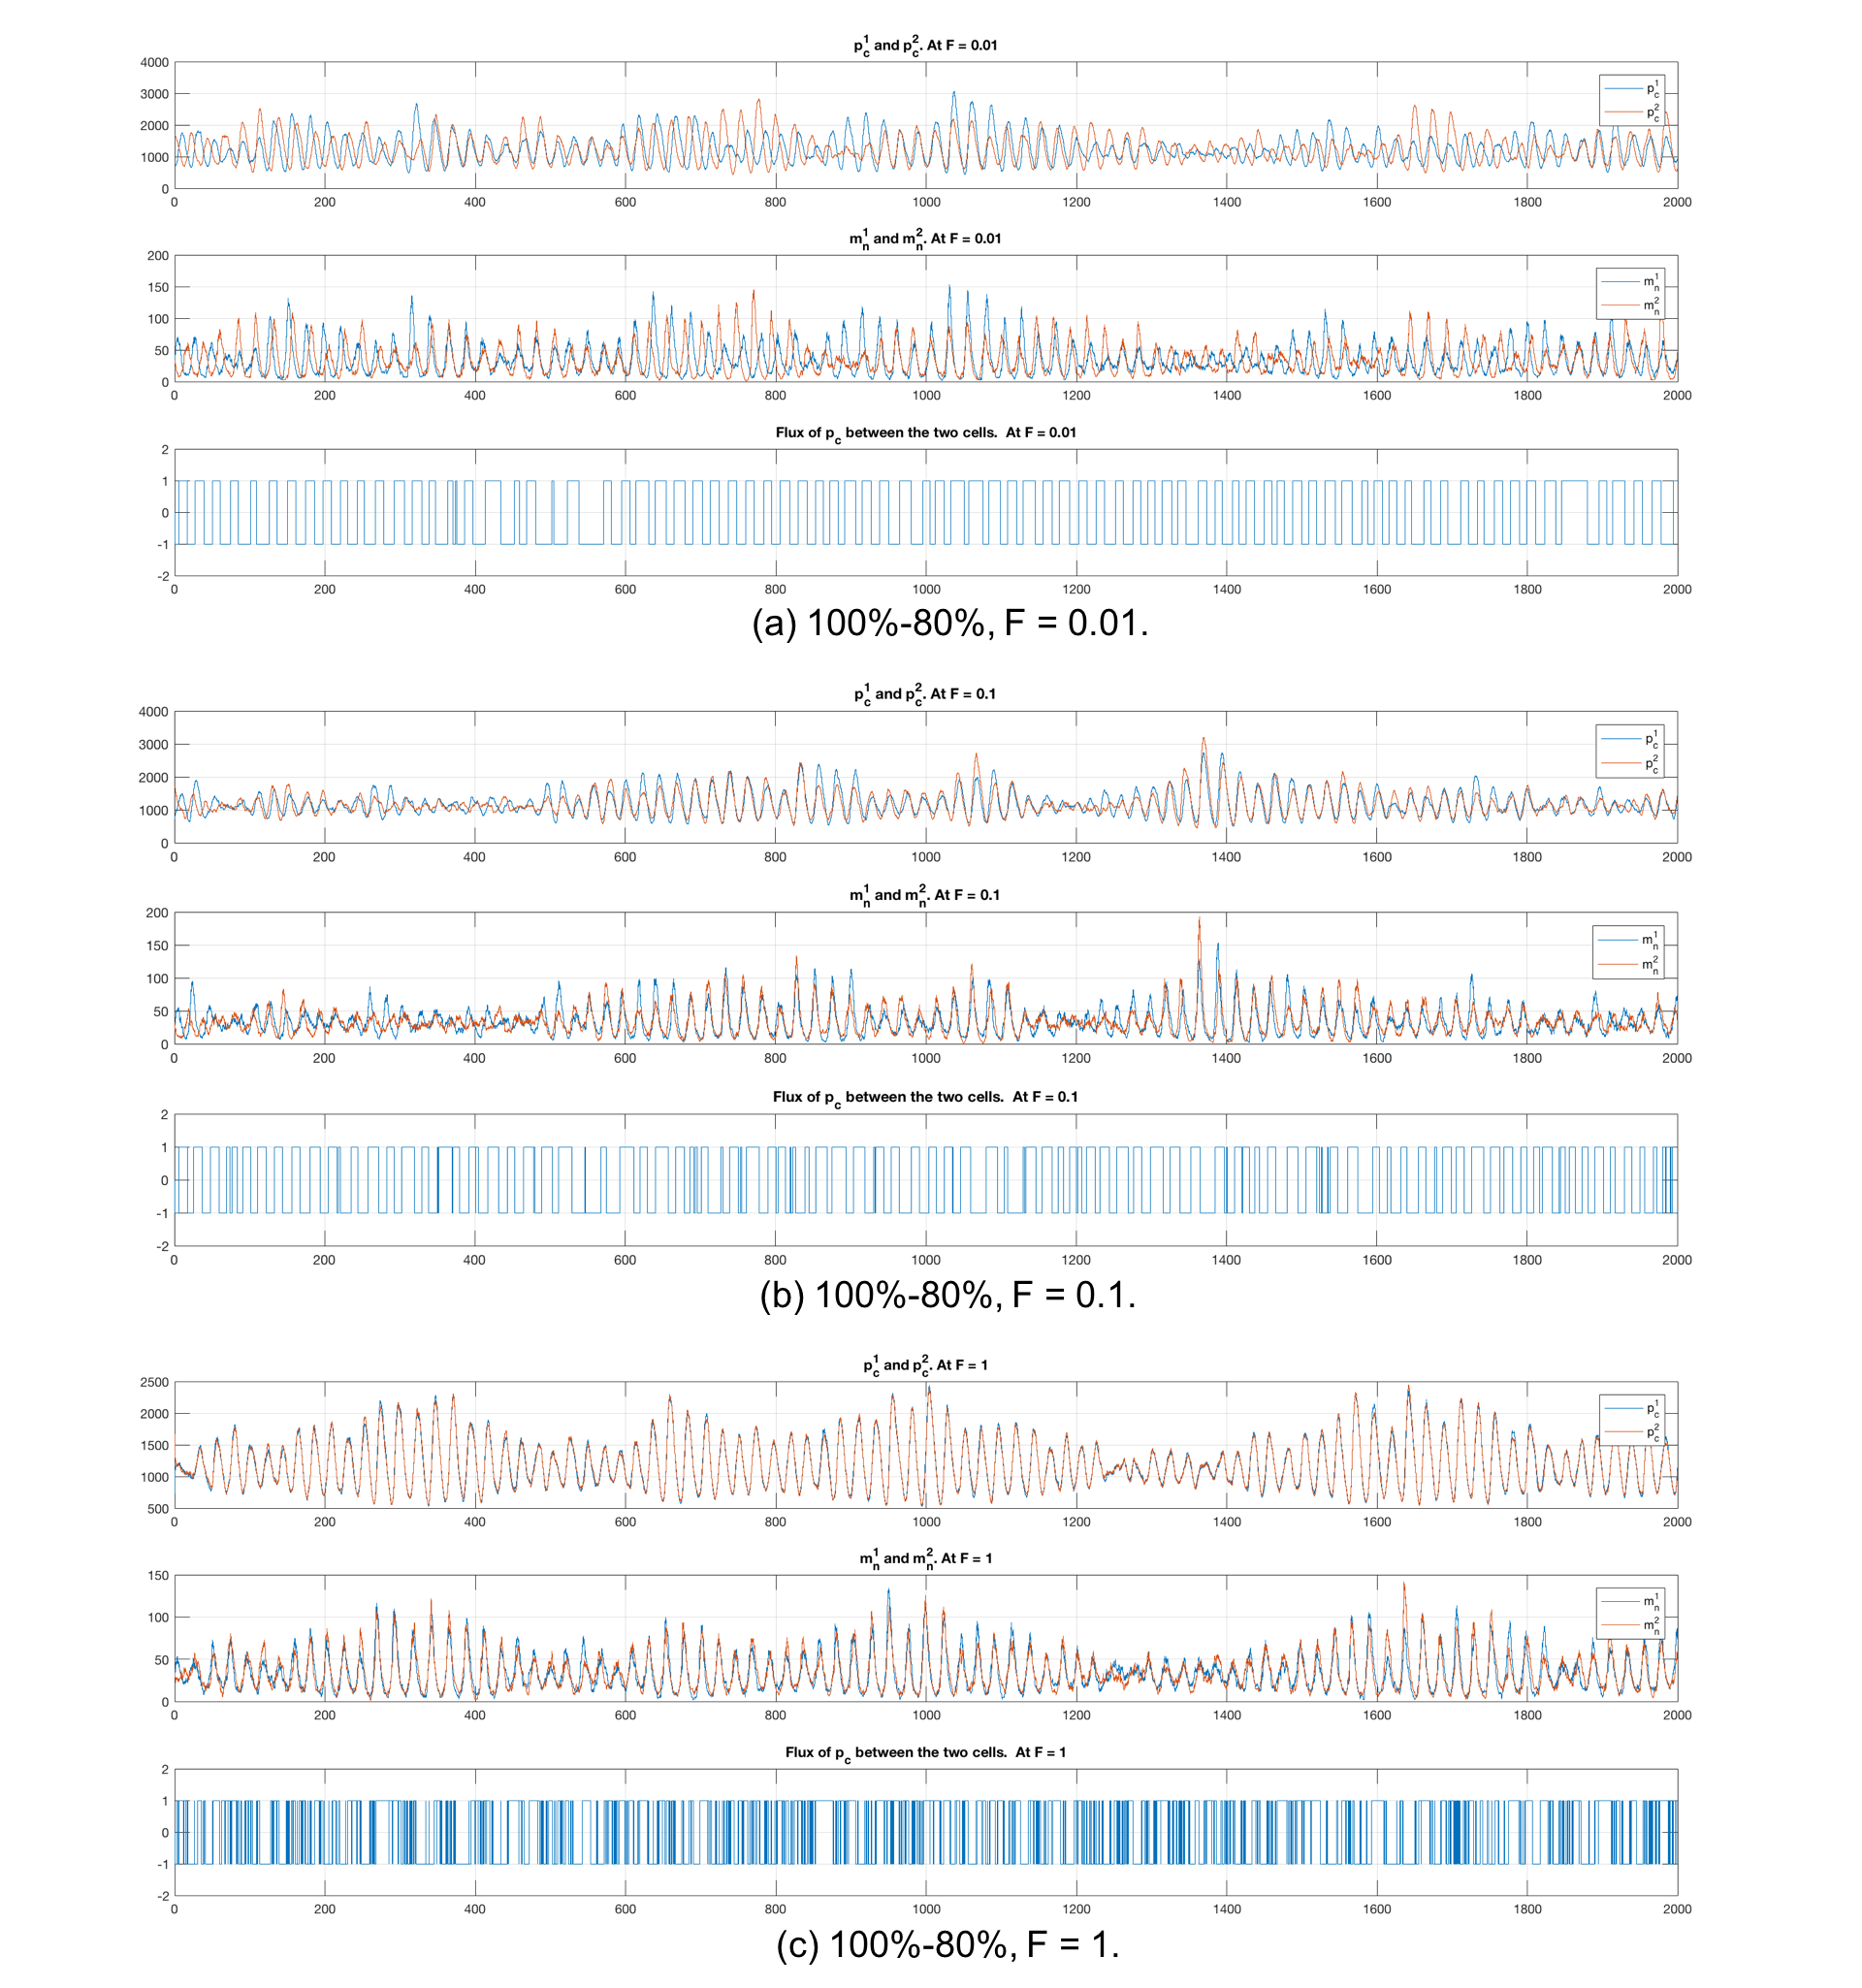
\includegraphics[width=0.99\textwidth]{sto_two_80_100_compare.png}
		\caption*{\small Figure X.}
	\end{minipage}
	\footnotesize
	\emph{Graphs are plotted for the stochastic version, with different values of $F.$ Cell 2 has a period of approximately 80\% of that of cell 1. The first and second plot in each graph are the number of proteins in cytoplasm and mRNAs in nucleus. The third plot is the flow of protein.}
\end{figure}

\textbf{Case 1:} The period of cell 2 is roughly 80\% of that of cell 1.

The results from the deterministic version of the model is shown in Figure X(a), (b) and (c). Observe that when $F$ is small ($F=0.01,$ Figure X(a)), the two oscillations do not converge. Since the flow of protein, $p_c,$ shows some repeated patterns, we are assured that sufficient amount of reaction time is given, as the system has become steady. One interesting result is when $F$ is set to $0.1,$ as is shown in Figure X(b). In this situation, with the introduction of protein flow, the oscillations in both cells get killed, and it seems that the joint system has reached a steady state. However, detailed equilibrium analysis is needed to fully understand this situation. When $F$ is large ($F = 1$ in Figure X(c)), we can see that the two different periods are converging. Although the two paths are not perfectly aligned, they are indeed matched. The corresponding stochastic versions are plotted in Figure X(a), (b) and (c). Results are similar, as when $F$ is small, hardly can we see any convergence. If $F$ is large enough, it is obvious that synchronization is successful. Here notice that Figure X(b) and Figure X(b) have identical parameters, with F being $0.1.$ But the results are vastly different: in the stochastic model, the oscillations are not killed, but instead some medium level of synchronization can be observed.



\textbf{Case 2:} The period of cell 2 is roughly 95\% of that of cell 1.

We expect that, if the innate difference between the two cells are small, then it should be easier to synchronize the two cells. Numerical results, as shown in Figure X(d), (e) and (f), confirm our expectation. Observe that in this case, $F=0.1$ would be large enough to generate a successful synchronization, while when $F=1,$ the synchronization is even faster.

Remark: If we compare the synchronization of identical cells with different initial states, with the synchronization of cells with innately different rhythms, we would see that the latter requires much faster flow of protein. In fact, $F$ needs to be at least 10 times larger, in order for cells with slightly different rhythms to get synchronized. This is intuitively clear, as synchronization of identical cells only requires the phases to be shifted, while synchronization of cells with different rhythms requires the flow of protein to fight against the original oscillation and transform the original rhythm.


\subsection{Two cellular oscillators with direct diffusion (ECF)}

\subsubsection{Unstable to Stable}

\subsubsection{Stable to Stable}

\subsubsection{Unstable to Unstable}

\subsubsection{Set of Eigenvalues with changing $\lambda_{ECF}$}

\begin{figure}[ht]
    \centering
	\begin{minipage}{0.99\textwidth}
		\centering
		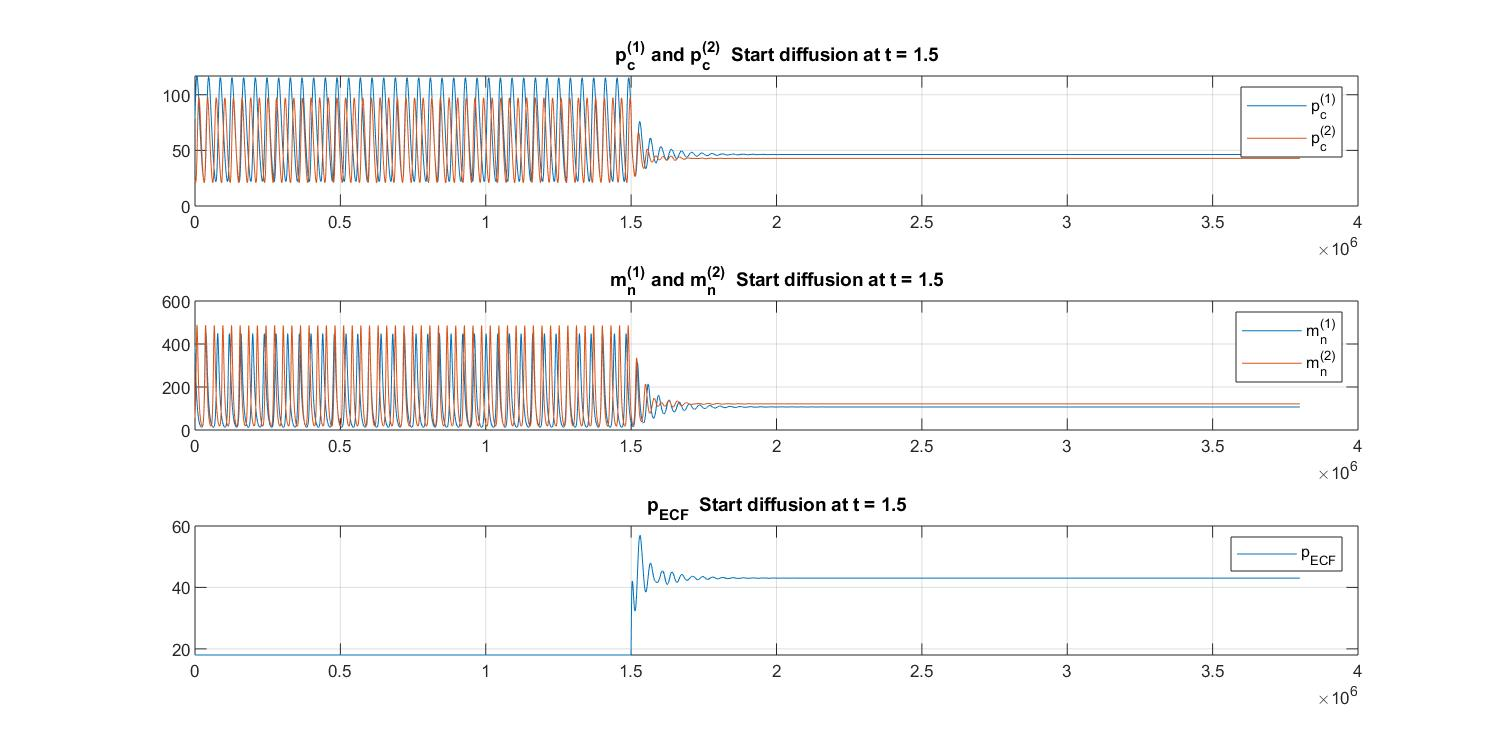
\includegraphics[width=0.8\textwidth]{US.jpg}
		\caption*{\small Figure}
	\end{minipage}
\end{figure}

\begin{figure}[ht]
    \centering
	\begin{minipage}{0.99\textwidth}
		\centering
		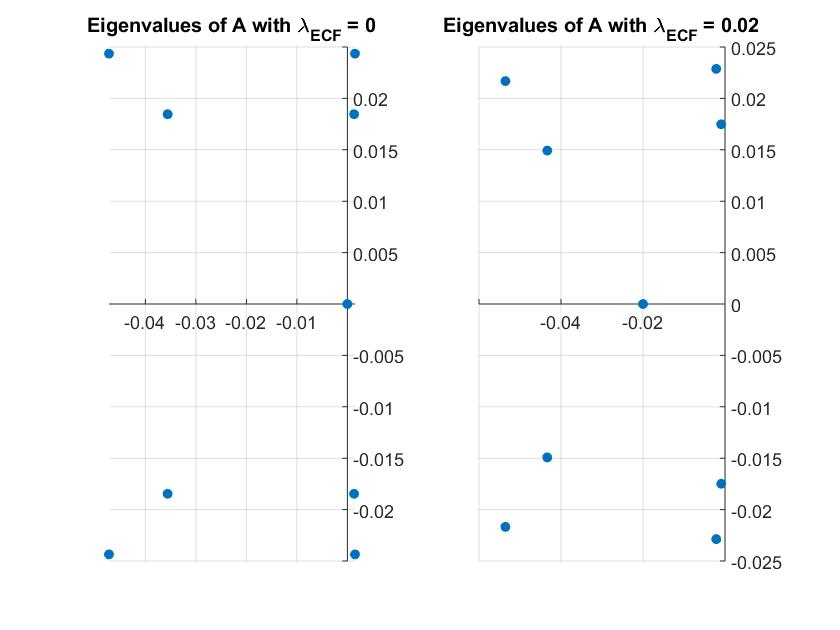
\includegraphics[width=0.8\textwidth]{USEi.jpg}
		\caption*{\small Figure}
	\end{minipage}
\end{figure}

\begin{figure}[ht]
    \centering
	\begin{minipage}{0.99\textwidth}
		\centering
		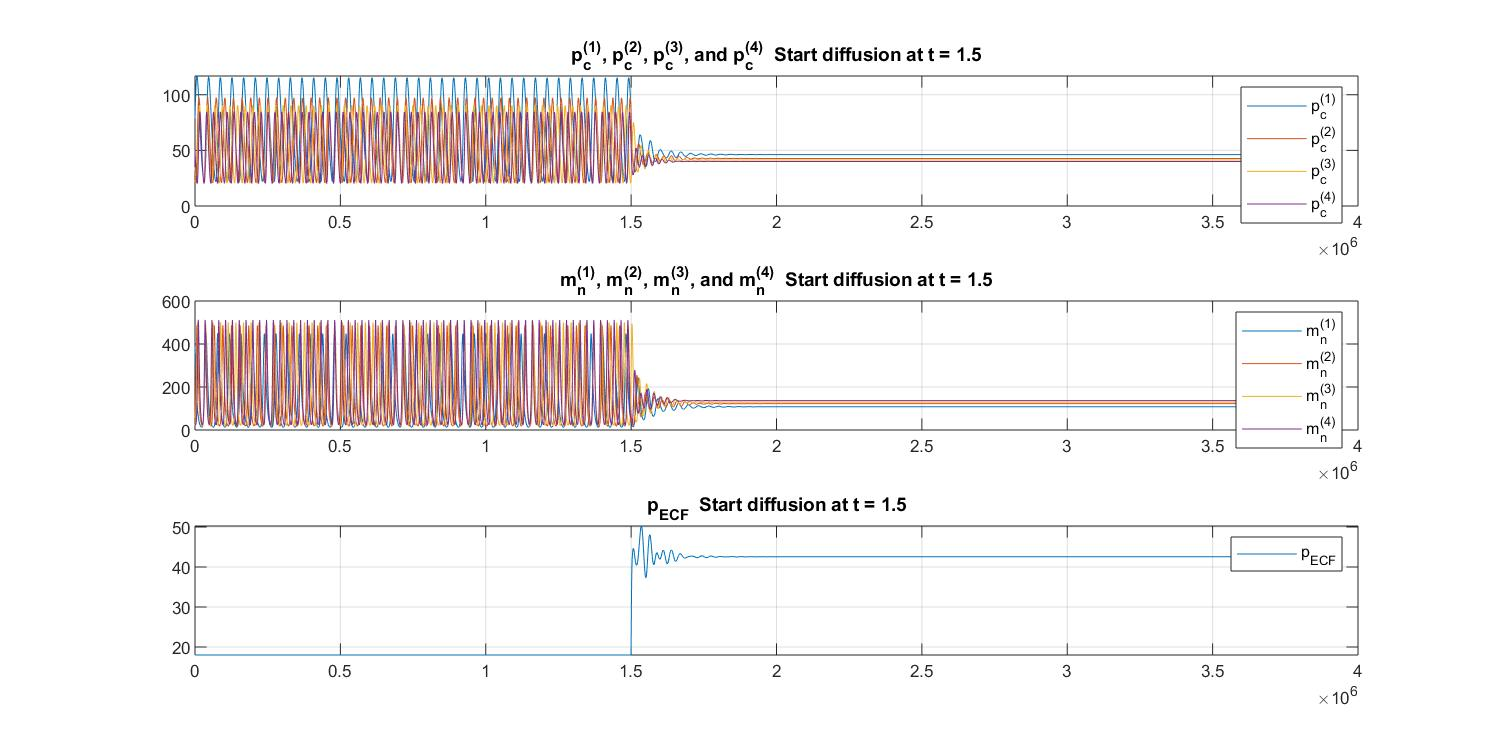
\includegraphics[width=0.8\textwidth]{US_M.jpg}
		\caption*{\small Figure}
	\end{minipage}
\end{figure}


\begin{figure}[ht]
    \centering
	\begin{minipage}{0.99\textwidth}
		\centering
		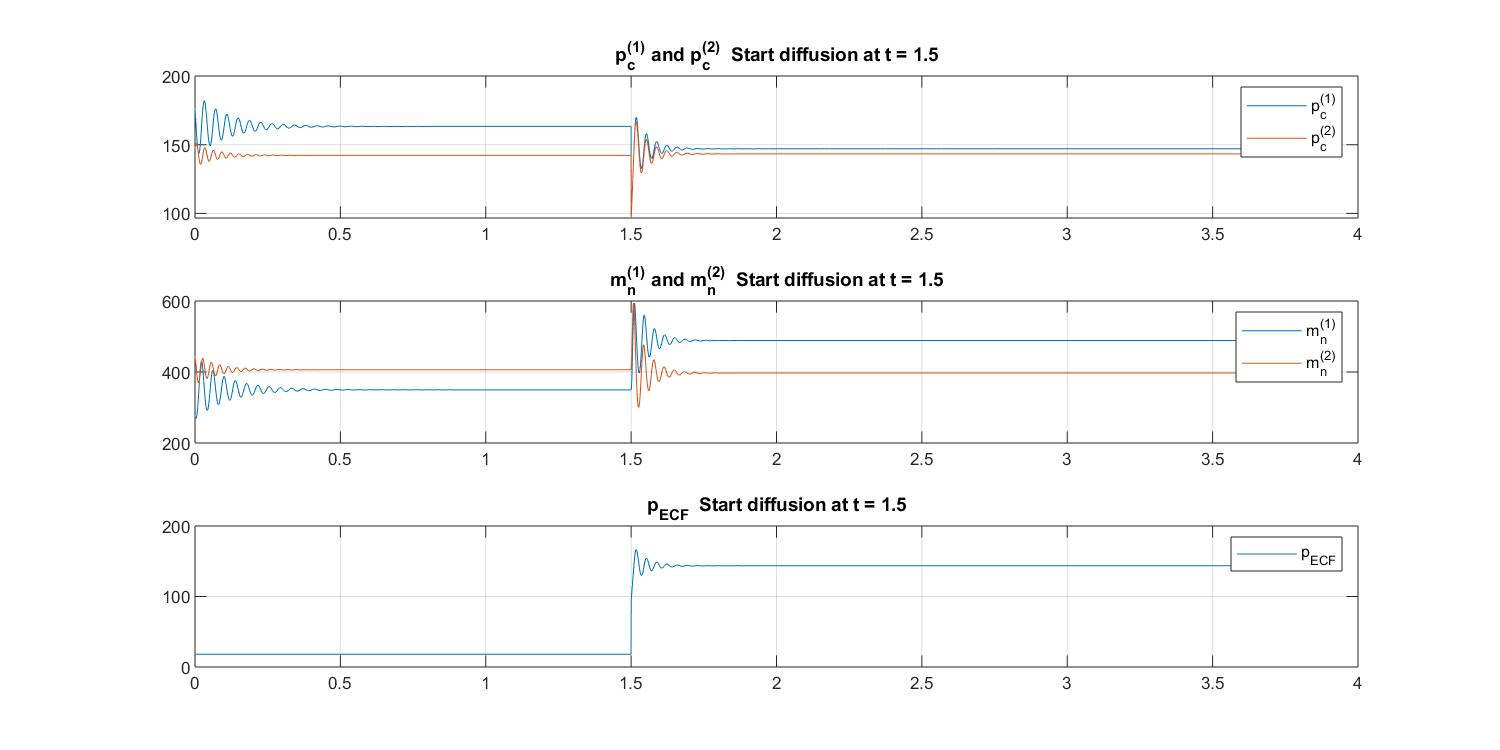
\includegraphics[width=0.8\textwidth]{SS.jpg}
		\caption*{\small Figure}
	\end{minipage}
\end{figure}

\begin{figure}[ht]
    \centering
	\begin{minipage}{0.99\textwidth}
		\centering
		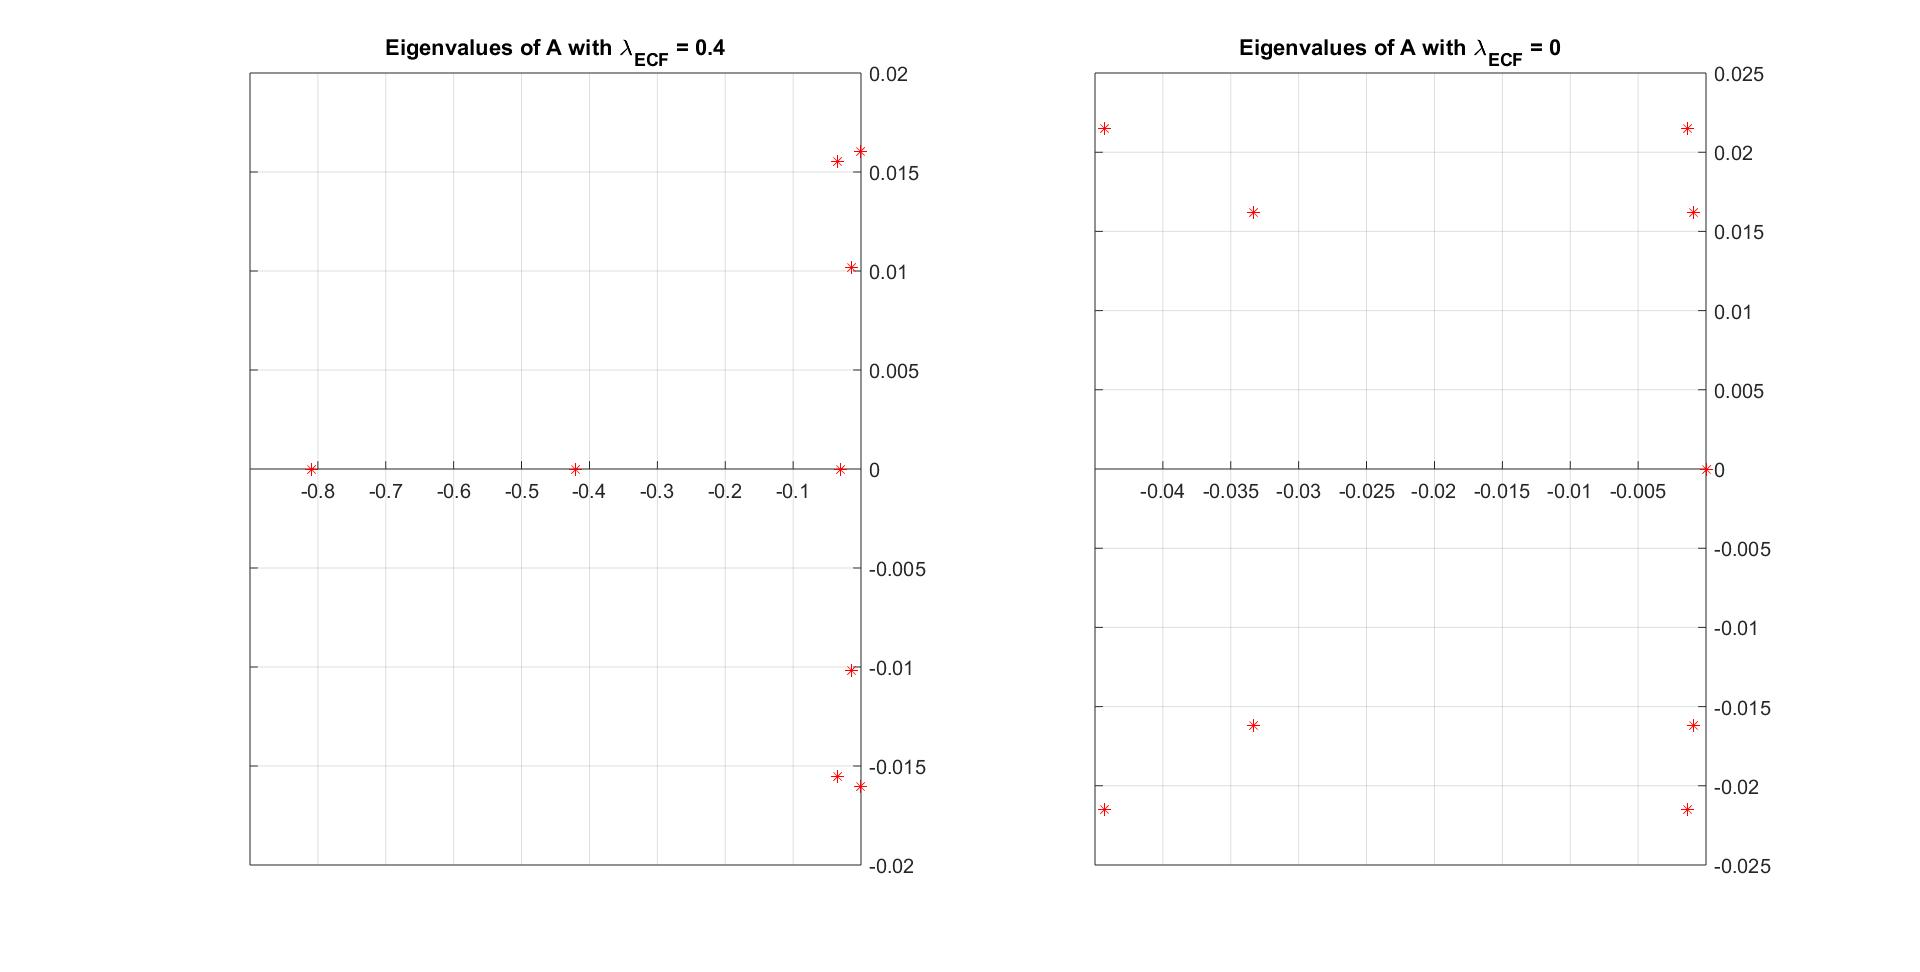
\includegraphics[width=0.8\textwidth]{SSEi.jpg}
		\caption*{\small Figure}
	\end{minipage}
\end{figure}

\begin{figure}[ht]
    \centering
	\begin{minipage}{0.99\textwidth}
		\centering
		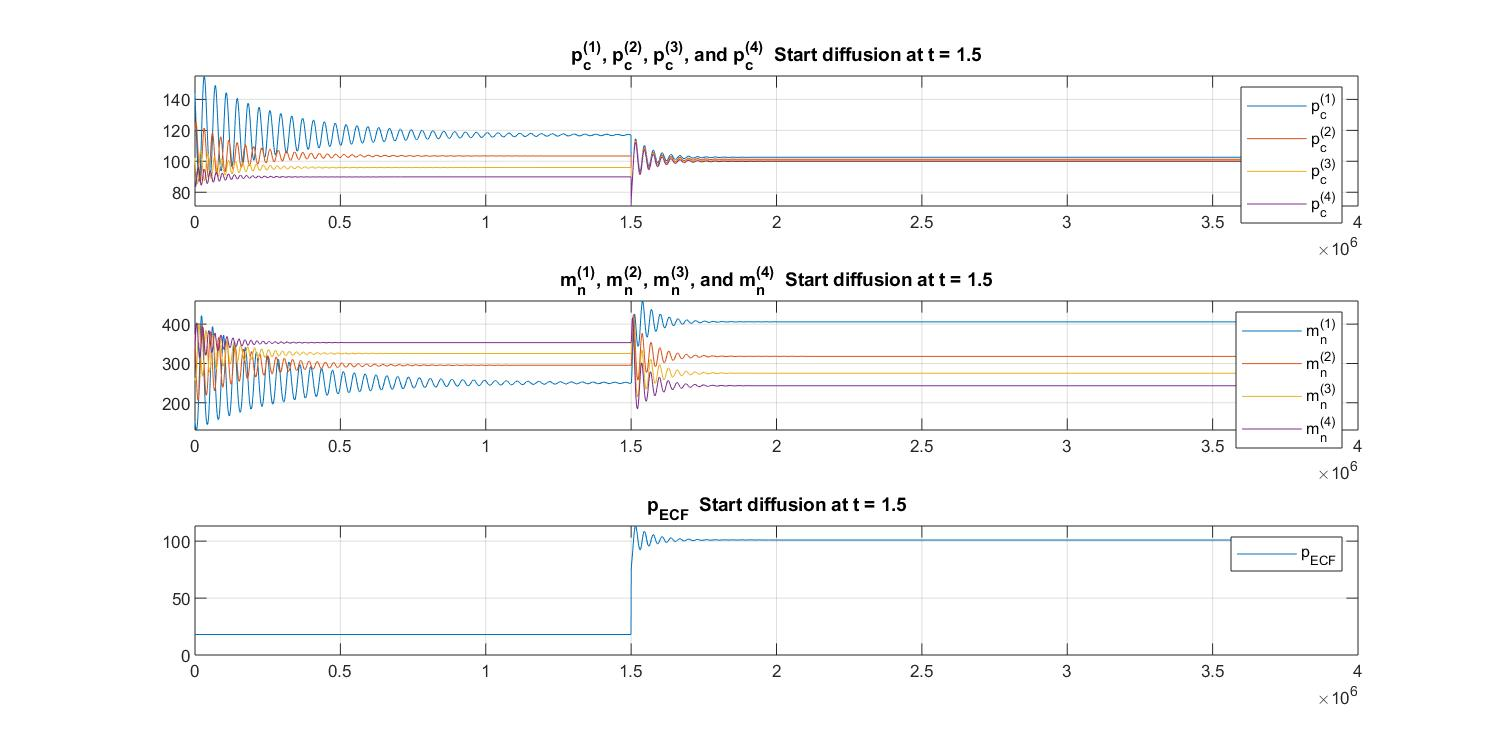
\includegraphics[width=0.8\textwidth]{SS_M.jpg}
		\caption*{\small Figure}
	\end{minipage}
\end{figure}


\begin{figure}[ht]
    \centering
	\begin{minipage}{0.99\textwidth}
		\centering
		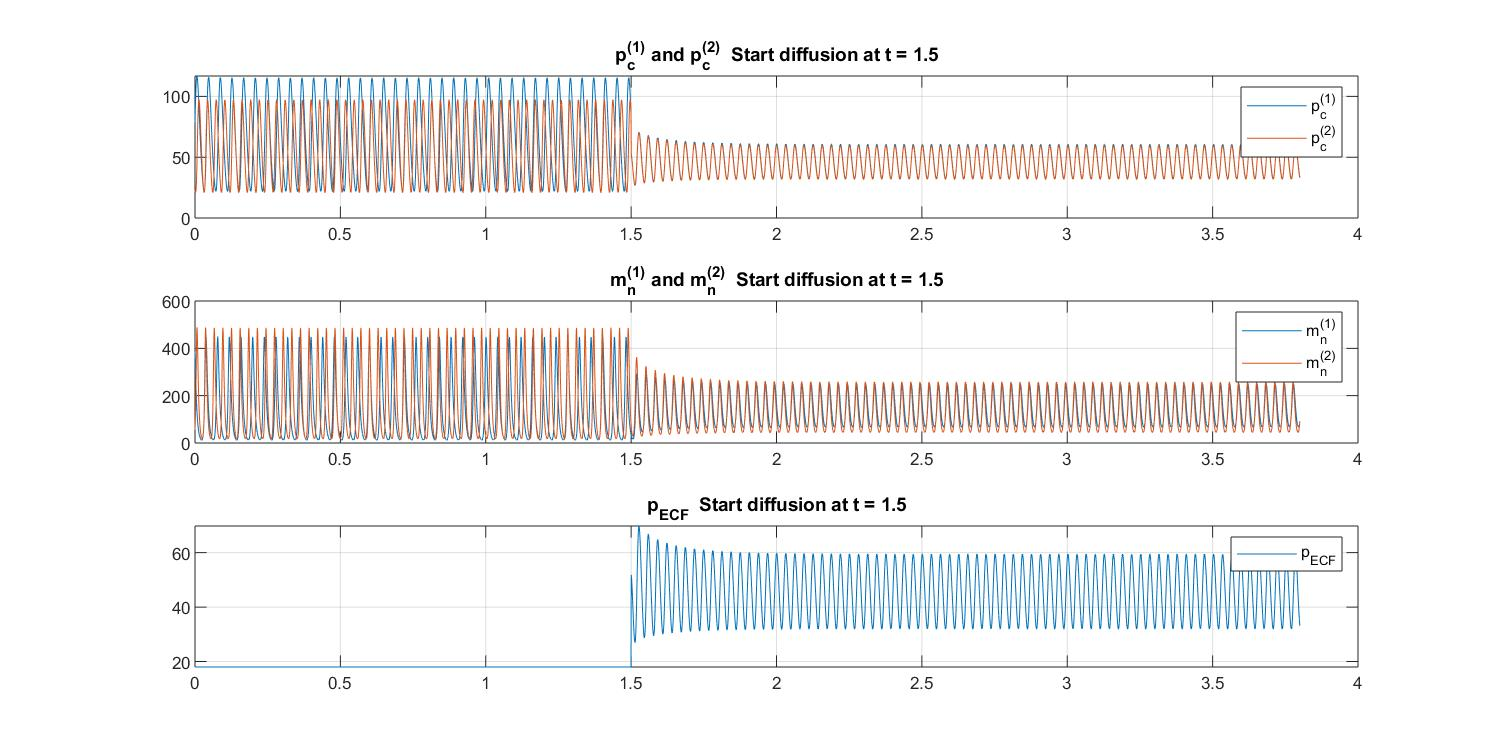
\includegraphics[width=0.8\textwidth]{UU.jpg}
		\caption*{\small Figure}
	\end{minipage}
\end{figure}

\begin{figure}[ht]
    \centering
	\begin{minipage}{0.99\textwidth}
		\centering
		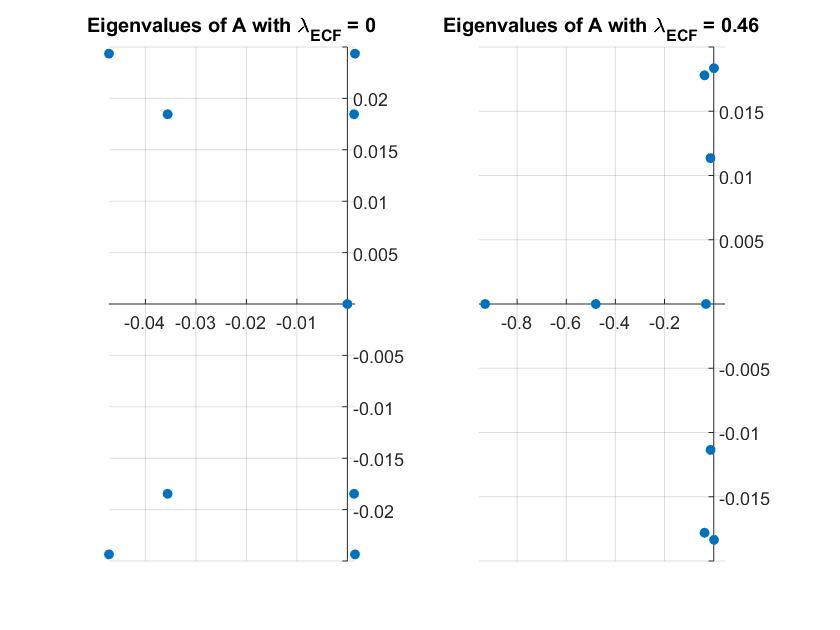
\includegraphics[width=0.8\textwidth]{UUEi.jpg}
		\caption*{\small Figure}
	\end{minipage}
\end{figure}

\begin{figure}[ht]
    \centering
	\begin{minipage}{0.99\textwidth}
		\centering
		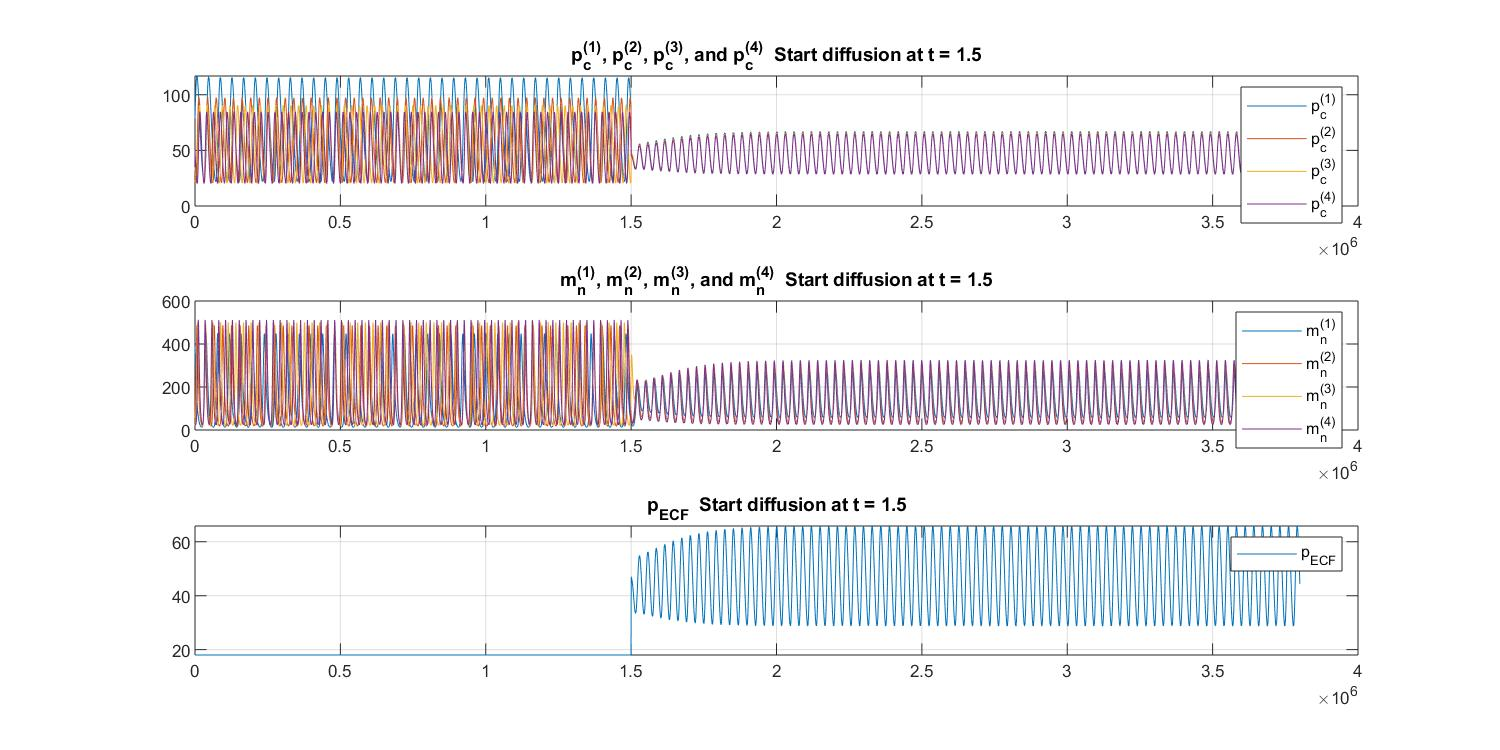
\includegraphics[width=0.8\textwidth]{UU_M.jpg}
		\caption*{\small Figure}
	\end{minipage}
\end{figure}

\begin{figure}[ht]
    \centering
	\begin{minipage}{0.99\textwidth}
		\centering
		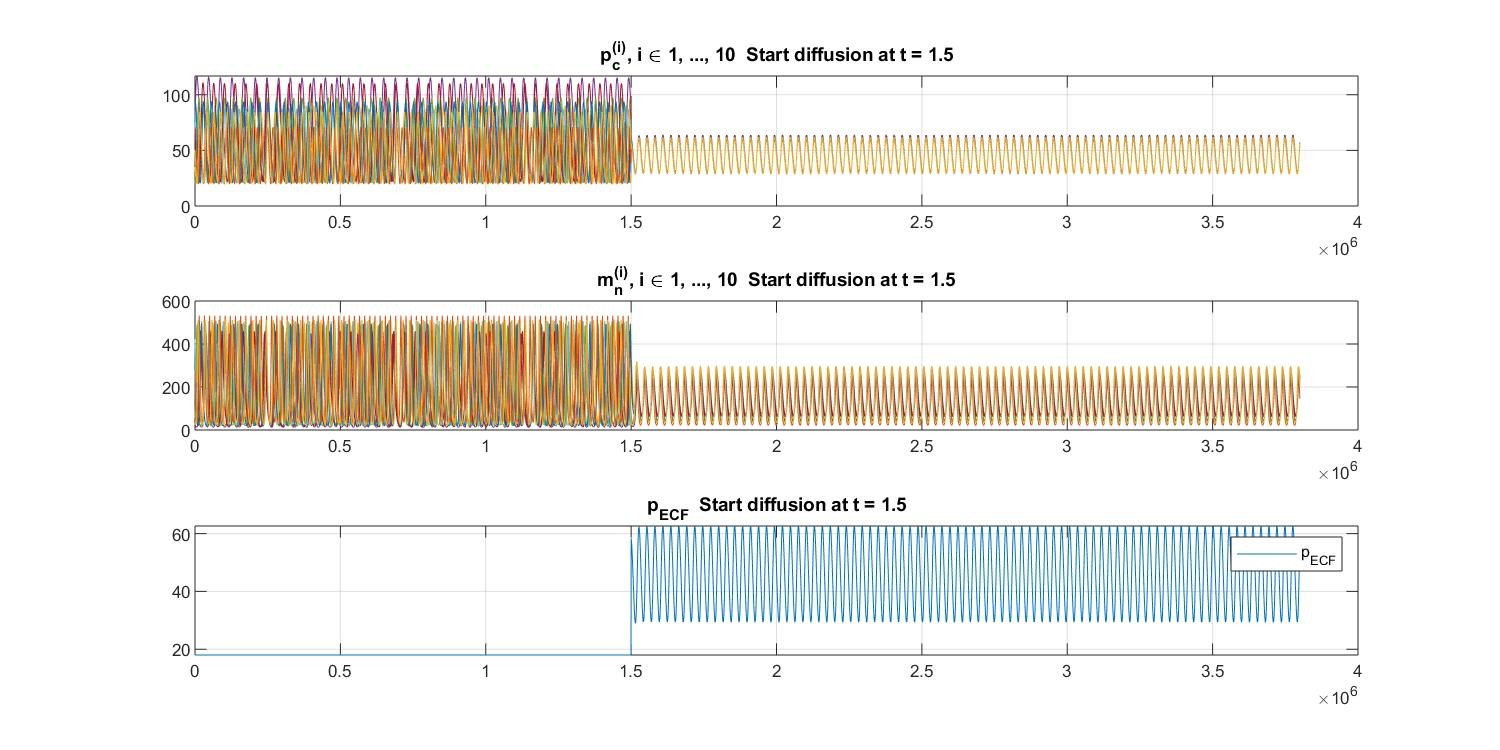
\includegraphics[width=0.8\textwidth]{UU_10.jpg}
		\caption*{\small Figure}
	\end{minipage}
\end{figure}

\begin{figure}[ht]
    \centering
	\begin{minipage}{0.99\textwidth}
		\centering
		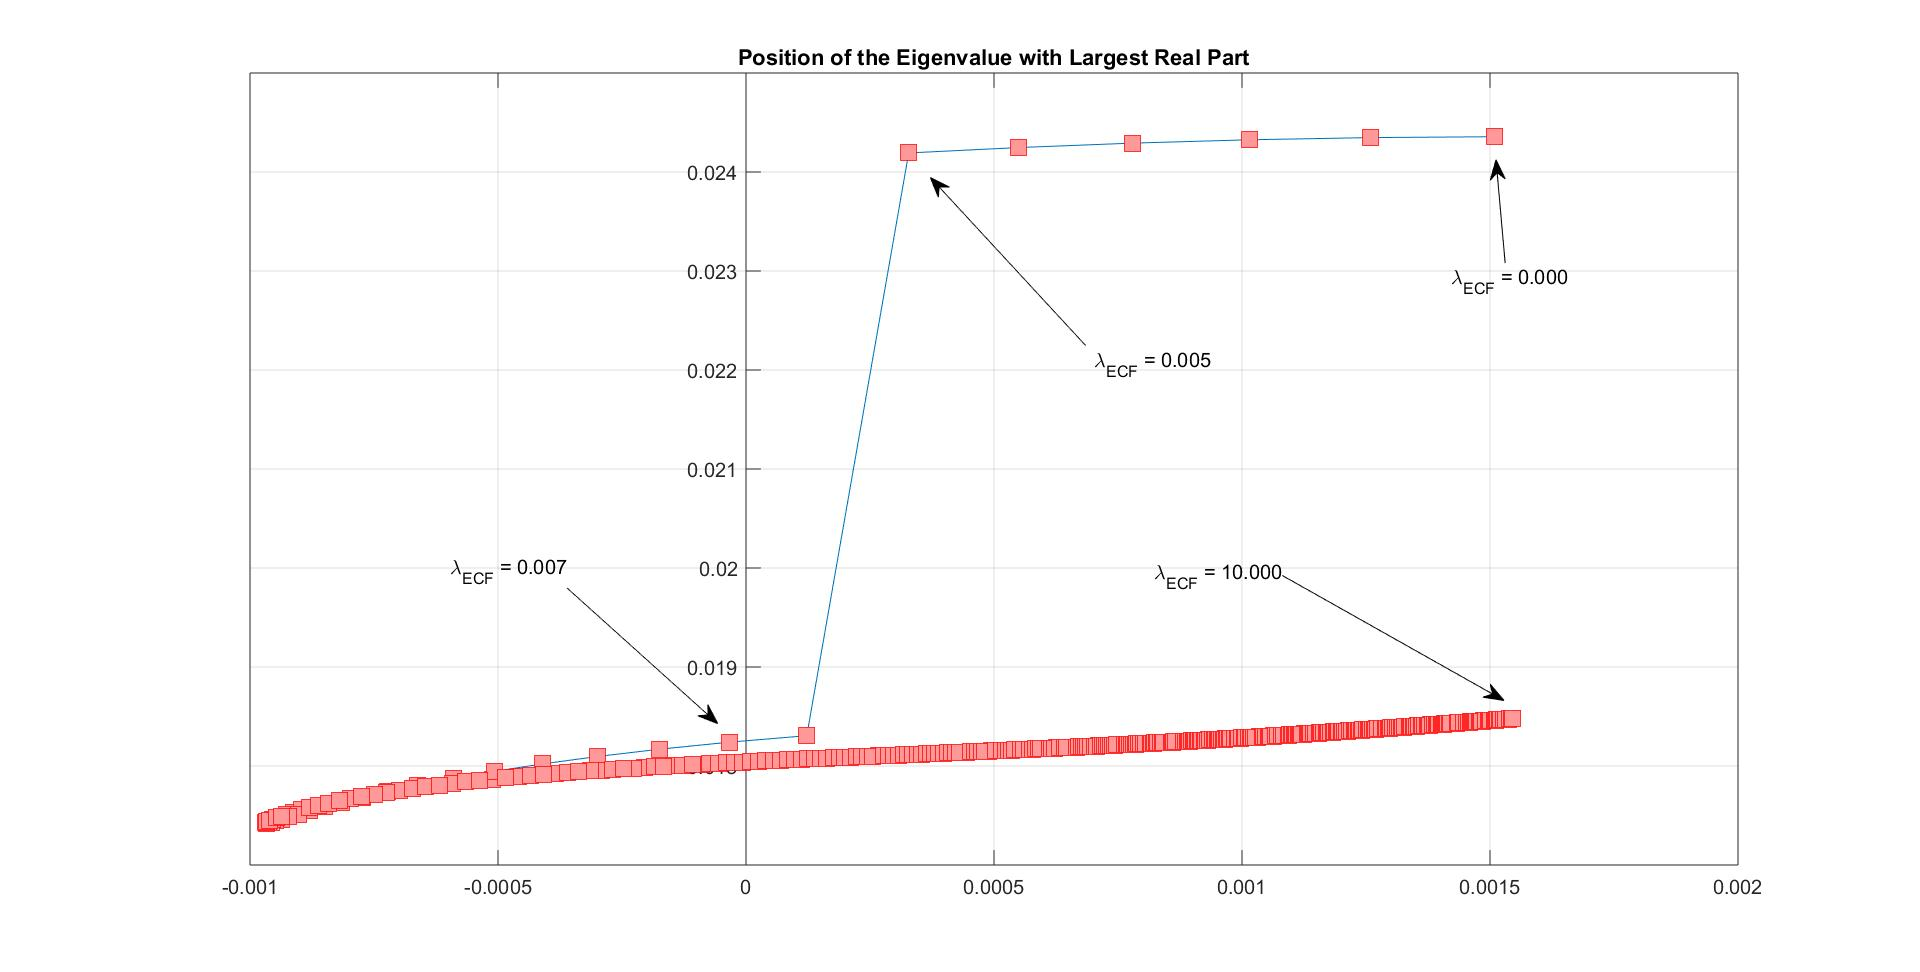
\includegraphics[width=0.8\textwidth]{all_lambda_Ei.jpg}
		\caption*{\small Figure}
	\end{minipage}
\end{figure}

\begin{figure}[ht]
    \centering
	\begin{minipage}{0.99\textwidth}
		\centering
		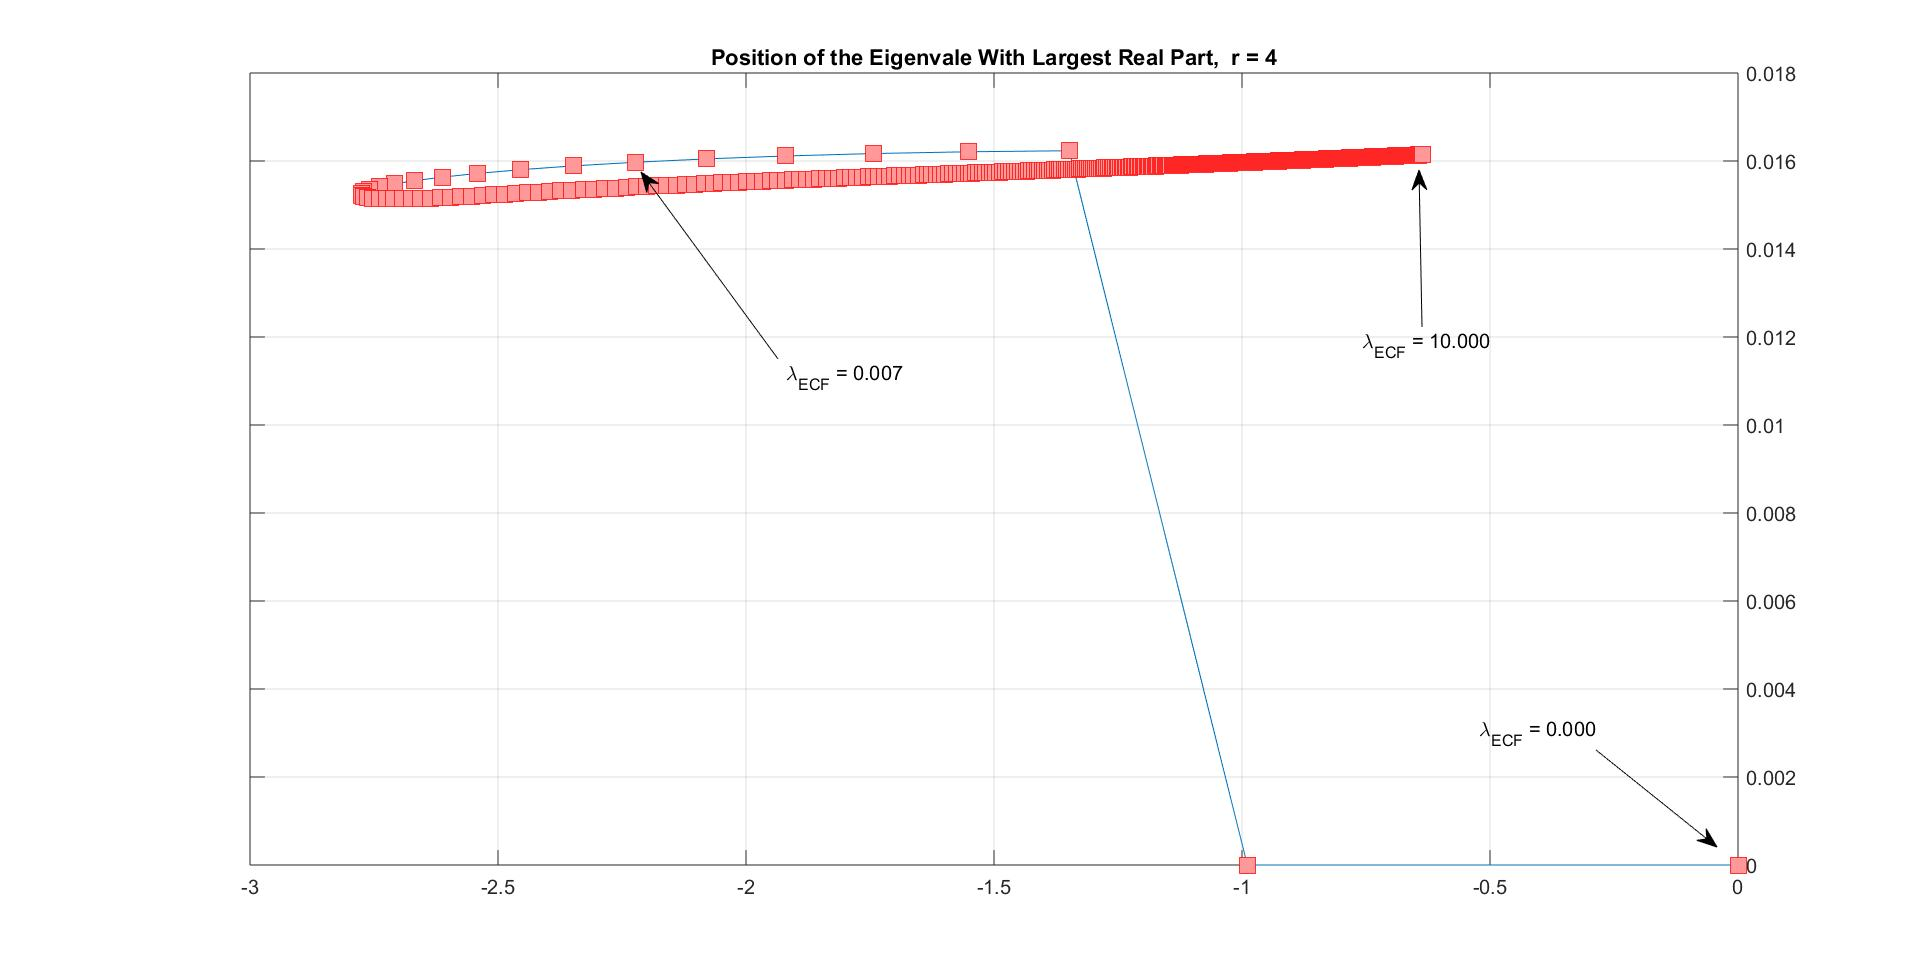
\includegraphics[width=0.8\textwidth]{all_lambda_Ei2.jpg}
		\caption*{\small Figure}
	\end{minipage}
\end{figure}



\begin{figure}[ht]
    \centering
	\begin{minipage}{0.99\textwidth}
		\centering
		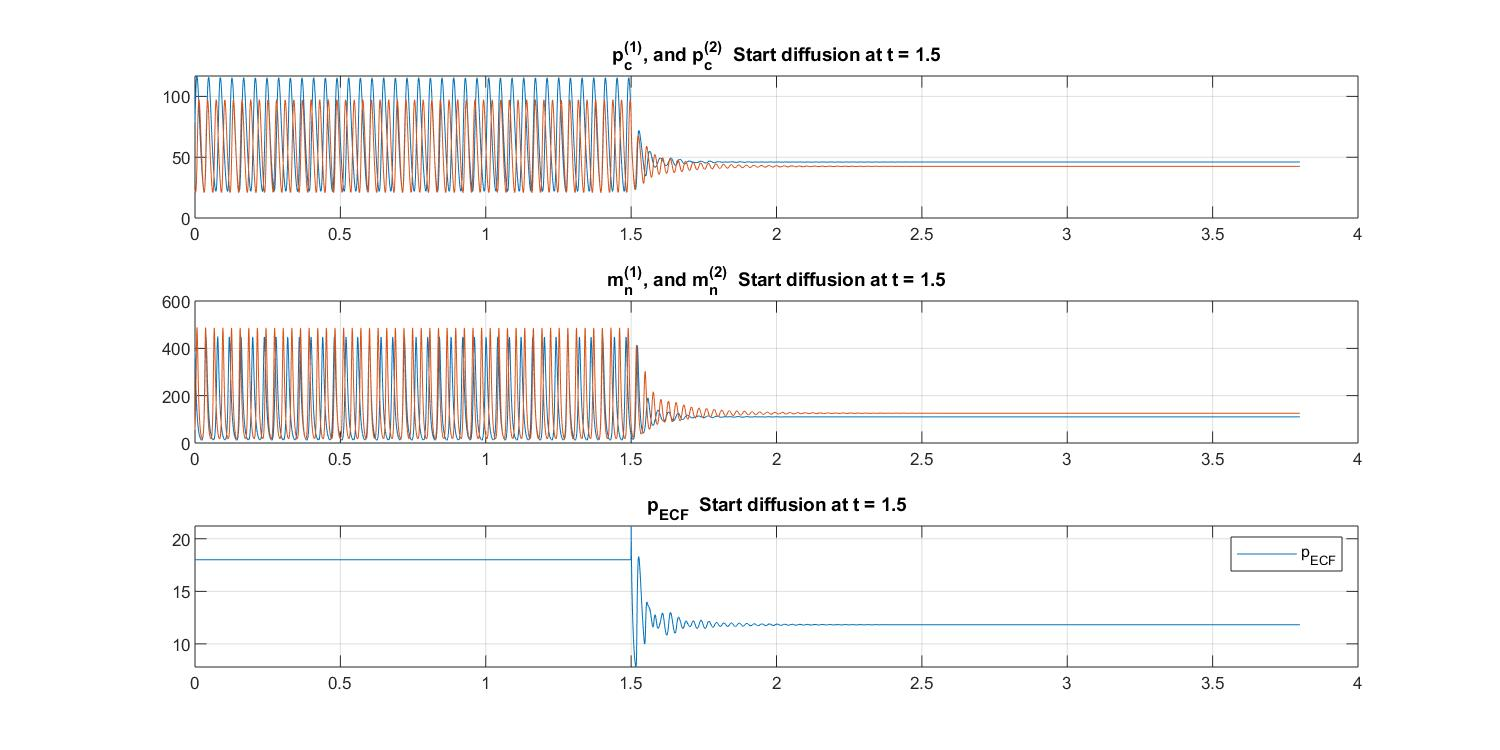
\includegraphics[width=0.8\textwidth]{PF_US.jpg}
		\caption*{\small Figure}
	\end{minipage}
\end{figure}


\begin{figure}[ht]
    \centering
	\begin{minipage}{0.99\textwidth}
		\centering
		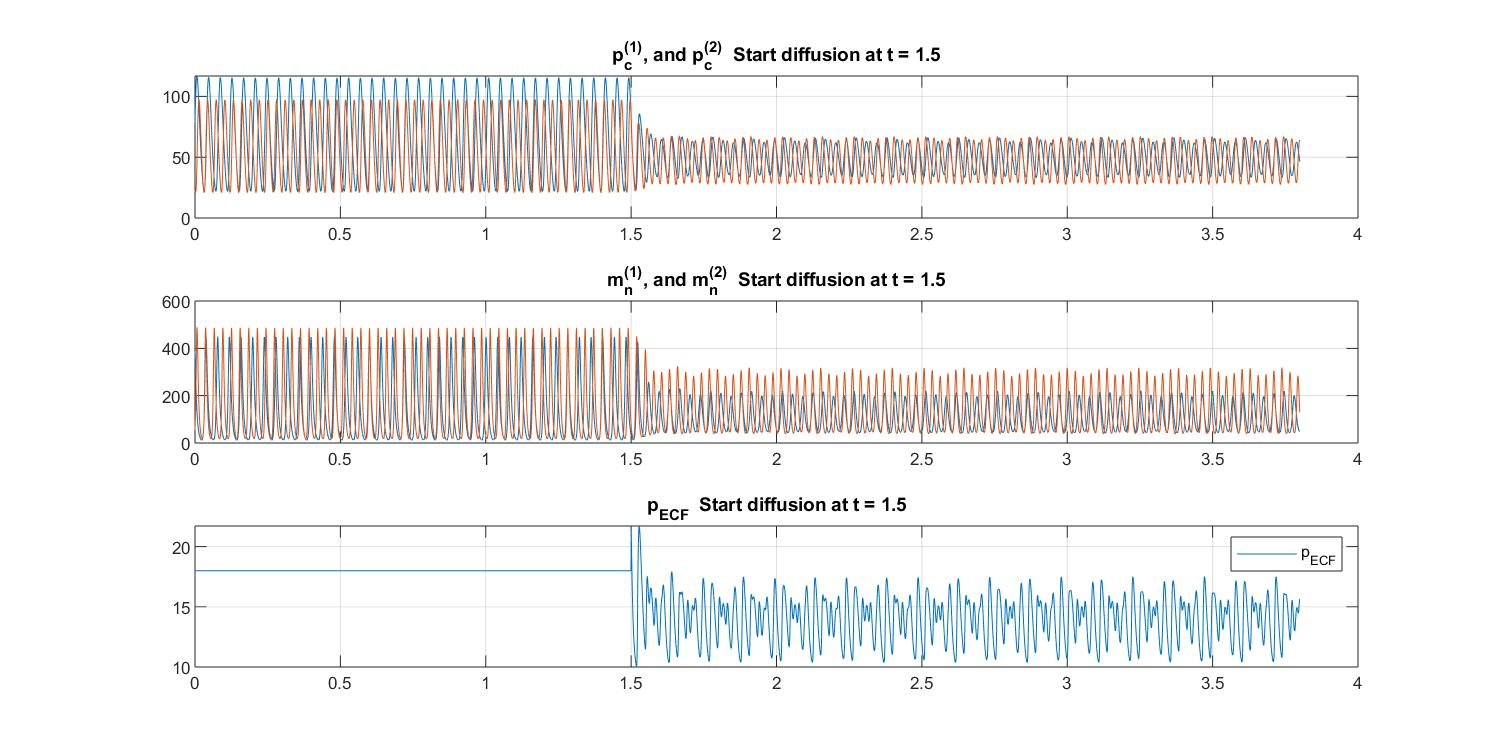
\includegraphics[width=0.8\textwidth]{PF_UU.jpg}
		\caption*{\small Figure}
	\end{minipage}
\end{figure}


\begin{figure}[ht]
    \centering
	\begin{minipage}{0.99\textwidth}
		\centering
		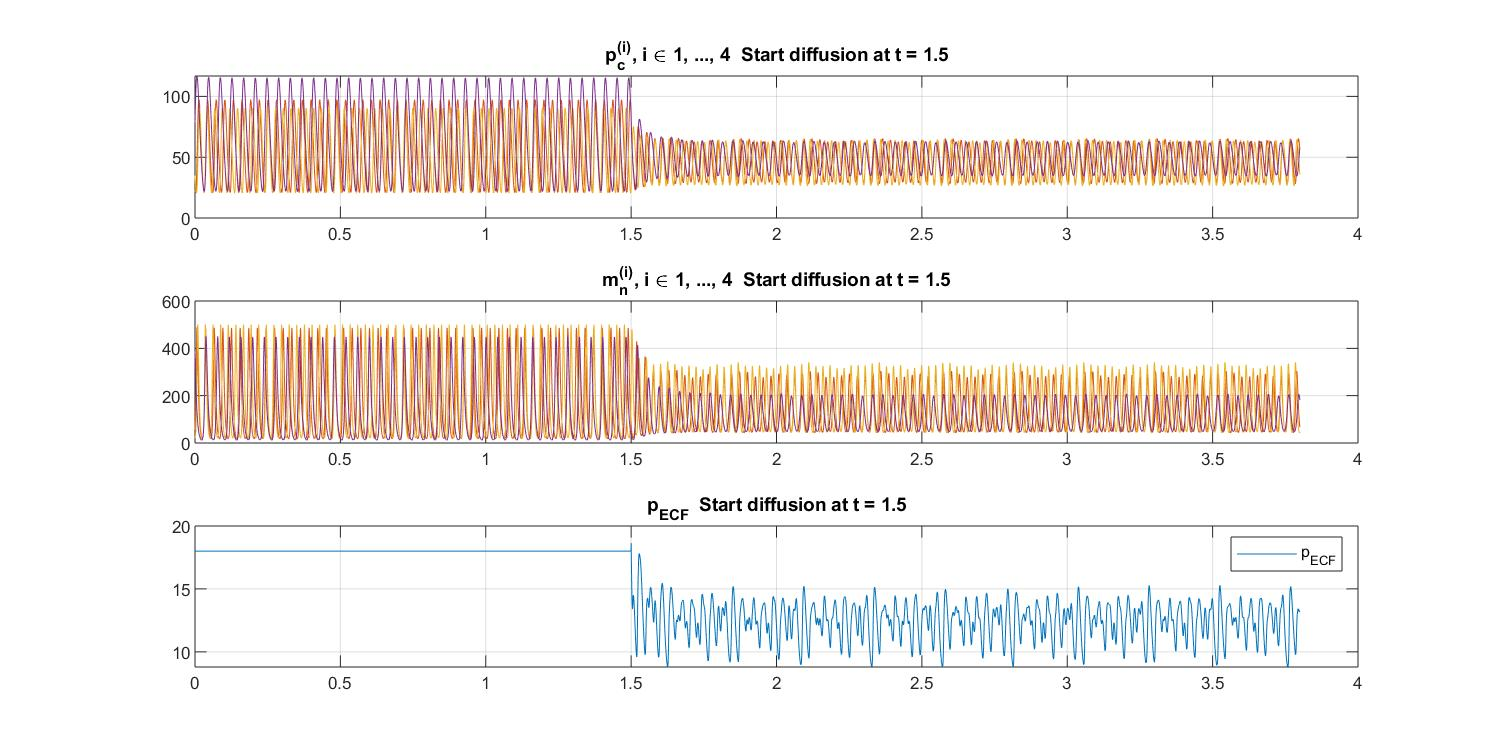
\includegraphics[width=0.8\textwidth]{PF_UU_4.jpg}
		\caption*{\small Figure}
	\end{minipage}
\end{figure}


\begin{figure}[ht]
    \centering
	\begin{minipage}{0.99\textwidth}
		\centering
		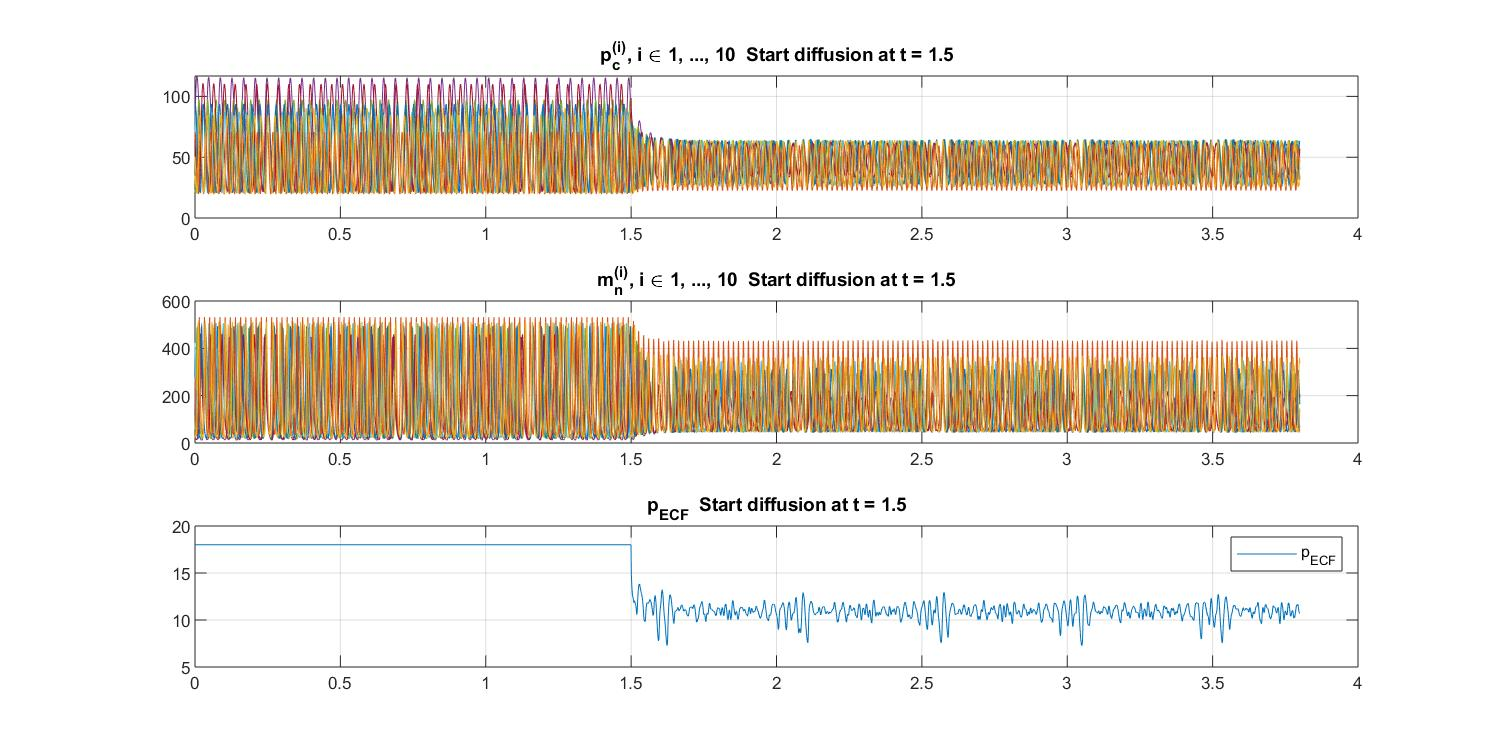
\includegraphics[width=0.8\textwidth]{PF_UU_10.jpg}
		\caption*{\small Figure}
	\end{minipage}
\end{figure}



\begin{comment}

\begin{thebibliography}{9}

	\bibitem{gyrocom}
	Charles S. Peskin. (2018).
	Notes on Physiological Control Mechanism.

	\bibitem{rbm}
	Charles Puelz. (2018).
	Matlab code about rigid body motion.




\end{thebibliography}
\end{comment}


\end{document}
